% Options for packages loaded elsewhere
\PassOptionsToPackage{unicode}{hyperref}
\PassOptionsToPackage{hyphens}{url}
\PassOptionsToPackage{dvipsnames,svgnames*,x11names*}{xcolor}
%
\documentclass[
  12pt,
  a4paper,
  oneside]{book}
\usepackage{lmodern}
\usepackage{setspace}
\usepackage{amssymb,amsmath}
\usepackage{ifxetex,ifluatex}
\ifnum 0\ifxetex 1\fi\ifluatex 1\fi=0 % if pdftex
  \usepackage[T1]{fontenc}
  \usepackage[utf8]{inputenc}
  \usepackage{textcomp} % provide euro and other symbols
\else % if luatex or xetex
  \usepackage{unicode-math}
  \defaultfontfeatures{Scale=MatchLowercase}
  \defaultfontfeatures[\rmfamily]{Ligatures=TeX,Scale=1}
\fi
% Use upquote if available, for straight quotes in verbatim environments
\IfFileExists{upquote.sty}{\usepackage{upquote}}{}
\IfFileExists{microtype.sty}{% use microtype if available
  \usepackage[]{microtype}
  \UseMicrotypeSet[protrusion]{basicmath} % disable protrusion for tt fonts
}{}
\makeatletter
\@ifundefined{KOMAClassName}{% if non-KOMA class
  \IfFileExists{parskip.sty}{%
    \usepackage{parskip}
  }{% else
    \setlength{\parindent}{0pt}
    \setlength{\parskip}{6pt plus 2pt minus 1pt}}
}{% if KOMA class
  \KOMAoptions{parskip=half}}
\makeatother
\usepackage{xcolor}
\IfFileExists{xurl.sty}{\usepackage{xurl}}{} % add URL line breaks if available
\IfFileExists{bookmark.sty}{\usepackage{bookmark}}{\usepackage{hyperref}}
\hypersetup{
  pdftitle={RUMAKI Seascape},
  pdfauthor={Baraka Kuguru},
  colorlinks=true,
  linkcolor=NavyBlue,
  filecolor=Maroon,
  citecolor=Blue,
  urlcolor=Blue,
  pdfcreator={LaTeX via pandoc}}
\urlstyle{same} % disable monospaced font for URLs
\usepackage[left=2.5cm, right=2.5cm, top=2.5cm, bottom=2.5cm]{geometry}
\usepackage{color}
\usepackage{fancyvrb}
\newcommand{\VerbBar}{|}
\newcommand{\VERB}{\Verb[commandchars=\\\{\}]}
\DefineVerbatimEnvironment{Highlighting}{Verbatim}{commandchars=\\\{\}}
% Add ',fontsize=\small' for more characters per line
\usepackage{framed}
\definecolor{shadecolor}{RGB}{248,248,248}
\newenvironment{Shaded}{\begin{snugshade}}{\end{snugshade}}
\newcommand{\AlertTok}[1]{\textcolor[rgb]{0.94,0.16,0.16}{#1}}
\newcommand{\AnnotationTok}[1]{\textcolor[rgb]{0.56,0.35,0.01}{\textbf{\textit{#1}}}}
\newcommand{\AttributeTok}[1]{\textcolor[rgb]{0.77,0.63,0.00}{#1}}
\newcommand{\BaseNTok}[1]{\textcolor[rgb]{0.00,0.00,0.81}{#1}}
\newcommand{\BuiltInTok}[1]{#1}
\newcommand{\CharTok}[1]{\textcolor[rgb]{0.31,0.60,0.02}{#1}}
\newcommand{\CommentTok}[1]{\textcolor[rgb]{0.56,0.35,0.01}{\textit{#1}}}
\newcommand{\CommentVarTok}[1]{\textcolor[rgb]{0.56,0.35,0.01}{\textbf{\textit{#1}}}}
\newcommand{\ConstantTok}[1]{\textcolor[rgb]{0.00,0.00,0.00}{#1}}
\newcommand{\ControlFlowTok}[1]{\textcolor[rgb]{0.13,0.29,0.53}{\textbf{#1}}}
\newcommand{\DataTypeTok}[1]{\textcolor[rgb]{0.13,0.29,0.53}{#1}}
\newcommand{\DecValTok}[1]{\textcolor[rgb]{0.00,0.00,0.81}{#1}}
\newcommand{\DocumentationTok}[1]{\textcolor[rgb]{0.56,0.35,0.01}{\textbf{\textit{#1}}}}
\newcommand{\ErrorTok}[1]{\textcolor[rgb]{0.64,0.00,0.00}{\textbf{#1}}}
\newcommand{\ExtensionTok}[1]{#1}
\newcommand{\FloatTok}[1]{\textcolor[rgb]{0.00,0.00,0.81}{#1}}
\newcommand{\FunctionTok}[1]{\textcolor[rgb]{0.00,0.00,0.00}{#1}}
\newcommand{\ImportTok}[1]{#1}
\newcommand{\InformationTok}[1]{\textcolor[rgb]{0.56,0.35,0.01}{\textbf{\textit{#1}}}}
\newcommand{\KeywordTok}[1]{\textcolor[rgb]{0.13,0.29,0.53}{\textbf{#1}}}
\newcommand{\NormalTok}[1]{#1}
\newcommand{\OperatorTok}[1]{\textcolor[rgb]{0.81,0.36,0.00}{\textbf{#1}}}
\newcommand{\OtherTok}[1]{\textcolor[rgb]{0.56,0.35,0.01}{#1}}
\newcommand{\PreprocessorTok}[1]{\textcolor[rgb]{0.56,0.35,0.01}{\textit{#1}}}
\newcommand{\RegionMarkerTok}[1]{#1}
\newcommand{\SpecialCharTok}[1]{\textcolor[rgb]{0.00,0.00,0.00}{#1}}
\newcommand{\SpecialStringTok}[1]{\textcolor[rgb]{0.31,0.60,0.02}{#1}}
\newcommand{\StringTok}[1]{\textcolor[rgb]{0.31,0.60,0.02}{#1}}
\newcommand{\VariableTok}[1]{\textcolor[rgb]{0.00,0.00,0.00}{#1}}
\newcommand{\VerbatimStringTok}[1]{\textcolor[rgb]{0.31,0.60,0.02}{#1}}
\newcommand{\WarningTok}[1]{\textcolor[rgb]{0.56,0.35,0.01}{\textbf{\textit{#1}}}}
\usepackage{longtable,booktabs}
% Correct order of tables after \paragraph or \subparagraph
\usepackage{etoolbox}
\makeatletter
\patchcmd\longtable{\par}{\if@noskipsec\mbox{}\fi\par}{}{}
\makeatother
% Allow footnotes in longtable head/foot
\IfFileExists{footnotehyper.sty}{\usepackage{footnotehyper}}{\usepackage{footnote}}
\makesavenoteenv{longtable}
\usepackage{graphicx,grffile}
\makeatletter
\def\maxwidth{\ifdim\Gin@nat@width>\linewidth\linewidth\else\Gin@nat@width\fi}
\def\maxheight{\ifdim\Gin@nat@height>\textheight\textheight\else\Gin@nat@height\fi}
\makeatother
% Scale images if necessary, so that they will not overflow the page
% margins by default, and it is still possible to overwrite the defaults
% using explicit options in \includegraphics[width, height, ...]{}
\setkeys{Gin}{width=\maxwidth,height=\maxheight,keepaspectratio}
% Set default figure placement to htbp
\makeatletter
\def\fps@figure{htbp}
\makeatother
% Make links footnotes instead of hotlinks:
\DeclareRobustCommand{\href}[2]{#2\footnote{\url{#1}}}
\setlength{\emergencystretch}{3em} % prevent overfull lines
\providecommand{\tightlist}{%
  \setlength{\itemsep}{0pt}\setlength{\parskip}{0pt}}
\setcounter{secnumdepth}{5}
\usepackage[none]{hyphenat}
\pagestyle{plain}
\raggedbottom 
\usepackage{booktabs}
\usepackage{makeidx}
\makeindex
\usepackage{titling}
\pretitle{\begin{center} 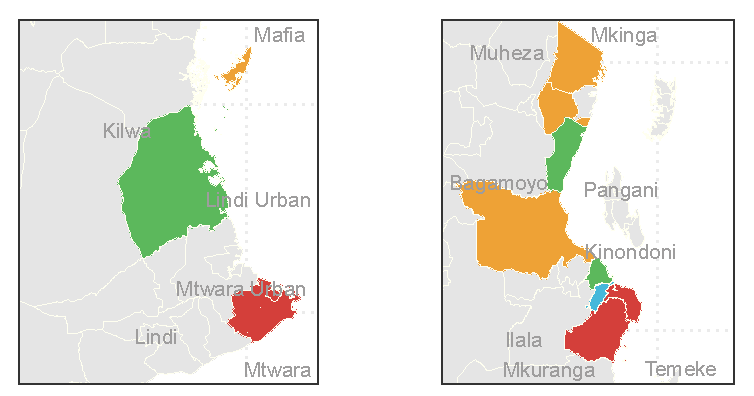
\includegraphics[width=6in,height=6in]{front.pdf}\LARGE\\}
\usepackage{float}
\floatplacement{figure}{H}
\renewcommand{\topfraction}{.85}
\renewcommand{\bottomfraction}{.7}
\renewcommand{\textfraction}{.15}
\renewcommand{\floatpagefraction}{.66}
\setcounter{topnumber}{3}
\setcounter{bottomnumber}{3}
\setcounter{totalnumber}{4}
\usepackage{fontspec}
\setmainfont{Adobe Caslon Pro}
\usepackage[utf8]{inputenc}
\hypersetup{unicode=true,pdfusetitle,bookmarks=true,bookmarksnumbered=true,bookmarksopen=true,bookmarksopenlevel=2,breaklinks=false,backref=false,colorlinks=true,linkcolor=blue}
\usepackage{booktabs}
\usepackage{longtable}
\usepackage{array}
\usepackage{multirow}
\usepackage{wrapfig}
\usepackage{float}
\usepackage{colortbl}
\usepackage{pdflscape}
\usepackage{tabu}
\usepackage{threeparttable}
\usepackage{threeparttablex}
\usepackage[normalem]{ulem}
\usepackage{makecell}
\usepackage{xcolor}
\usepackage[]{natbib}
\bibliographystyle{apalike}

\title{RUMAKI Seascape}
\usepackage{etoolbox}
\makeatletter
\providecommand{\subtitle}[1]{% add subtitle to \maketitle
  \apptocmd{\@title}{\par {\large #1 \par}}{}{}
}
\makeatother
\subtitle{Five Year Small Scale Fisheries Statistics (2014-2018)}
\author{Baraka Kuguru}
\date{June 2020}

\begin{document}
\maketitle

\begin{titlepage}
\vspace * {-2.5cm}	
	WWF\textcopyright2020\\
	The Fisheries Statistics of\\
	RUMAKI Seascape\\
	Project - e--CAS for Fisheries Data Records
	
\begin{center}

\vspace * {5cm}
%\huge \textbf{e--CAS for Fisheries Data Records}
\huge \textbf{e--CAS for Fisheries Data Records}

%\huge \textbf{e--CAS for Fisheries Data Records}
%
%\vspace * {1cm}
%
%\large \textbf{Kagera River}

%\huge e--CAS for Fisheries Data Records

\vspace * {2cm}
%\begin{figure}[htp]
%	\centering
%	\includegraphics[width=11cm]{kagera.jpg}
%\end{figure}

%\vspace * {2cm}
\large
WWF - Dar es Salaam\\ 

%\vspace * {4cm}
\large
Dar es Salaam, June 2020\\ 


\end{center}


\end{titlepage}

{
\hypersetup{linkcolor=}
\setcounter{tocdepth}{1}
\tableofcontents
}
\listoftables
\listoffigures
\setstretch{1.2}
\hypertarget{executive-summary}{%
\chapter*{Executive Summary}\label{executive-summary}}
\addcontentsline{toc}{chapter}{Executive Summary}

It is widely recognized that knowledge of the status and trends of capture fisheries, including socio--economic aspects, is a key to sound policy--development, better decision--making and responsible fisheries management. For the fisheries to contribute to food security it is important that information related to a particular stock or entire fisheries is available on an instant basis. Countries in coastal East Africa have taken up a scheme to decentralized management of the fisheries. These countries have introduced fisheries co--management systems---approach to manage coastal and marine resources. It was anticipated that participation of BMUs in the data collection would improve coverage and timely collection of the fisheries data.\index{fisheries!statistics}

In 2016, TAFIRI in collaboration with WWF conducted a pilot study to explore the use of the mobile application as a tool in fisheries data collection (e--CAS). The initiative started with five (5) selected BMUs. Members were trained on the use of mobile application in fisheries data collection. It was through this initiative species of tuna and tuna-like were recorded for the first time \citep{kuguru}. As of today, the initiative was expanded to to all coastal districts landing sites in Mainland Tanzania and endorsed by the Government. The current assignment aimed to analyze data collected from the e-CAS and regular CAS survey collected from 2014 to 2018 to assess stock healthiness and quality of small-scale fisheries landings in Rufiji \index{RUMAKI!Rufiji}, Mafia \index{RUMAKI!Mafia}, and Kilwa \index{RUMAKI!Kilwa} districts (RUMAKI). \index{RUMAKI}

The status of fish stock healthiness in the RUMAKI and Non--RUMAKI districts was assessed based on the data from CAS spanning from 2014 to 2018 and additional data from the e--CAS \index{Tools!e--CAS} spanning from 2016 to 2019 respectively. Fisheries catch\index{fisheries!catch} variation spatial maps, total catch and catch trends of the six priority fishery categories were used to assess the status of fish stock healthiness in the RUMAKI districts. The report focus on major five priority fisheries groups due the reasons that there was inconsistent in the data collection in terms of specific species or particular family groups. The groups were drawn from the ongoing SWIOFISH project. These include \emph{Octopus}\index{Family!octopus}, \emph{Small pelagics}\index{Family!pelagics}, \emph{tuna and tuna} like species\index{Family!tuna}, \emph{Reef} \index{Family!reef} and \emph{Elasmobranch}\index{Family!elasmobrach} species.\index{Non--RUMAKI}

The average annual total catch for the octopus fishery was found to be 124.83 \(\pm\) 16.33 tones per year in the non-RUMAKI and 173.90 \(\pm\) 20.77 (*Mean \(\pm\) SD) tones per year in the RUMAKI districts (Appendix \ref{tab:tab071}); the district of Kilwa and Ilala had higher landings in the RUMAKI and no-RUMAKI respectively (Appendix \ref{tab:tab072}). For tuna and tuna-like, the average total annual catch for the tuna and tuna-like species was found to be 74.85 \(\pm\) 8.28 tones per year in the non-RUMAKI and 65.55 \(\pm\) 10.51 tones per year in the RUMAKI districts (Appendix \ref{tab:tab071}. The Ilala district had higher landings in Non--RUMAKI and in the RUMAKI and Mafia had the highest catch in RUMAKI (Appendix \ref{tab:tab072}). The average annual total catch for the Small pelagic fishery was found to be 153.25 \(\pm\) 17.32 tones per year in the non-RUMAKI and 121.21 \(\pm\) 20.82 tones per year in the RUMAKI districts; the Mkuranga and Mtwara rural districts had higher landings in the RUMAKI and no-RUMAKI respectively (Appendix \ref{tab:tab072}). In addition, for reef species the average annual landing was found to be 113.83 \(\pm\) 17.93 tones per year in the non-RUMAKI and 102.87 \(\pm\) 21.85 tones per year in the RUMAKI districts (Appendix \ref{tab:tab071}); the Mafia and Pangani districts had higher landings in the RUMAKI and no-RUMAKI respectively (Appendix \ref{tab:tab072}).

In general, findings indicate there is a decrease in total catch from artisanal fishers in the RUMAKI districts for all major fisheries groups with the exception of small pelagic based on the data collected by BMUs from 2016-2019. Data collection is improving, in terms of timely submission of the data, but there is inconsistency in the data collection and little focus on the species of interest.

Among others, the current report recommended the following: The Department of Fisheries (DoF) \index{Institutes!Department of Fisheries} in collaboration with TAFIRI \index{Institutes!TAFIRI} should consider identifying representative species for all priority (major) fisheries groups and consistency follow up the data collection on the identified species. The DoF should consider adapting and upscaling the eCAS as the main data collection tool. Promote timely preparation of fishery statistics through the application of the databases. This should go along with the timely sharing of the statistics with relevant stakeholders. In addition, promote capacity development to all levels in the area of data collection, processing, analysis, interpretation and reporting. This should go hand in hand with periodic strategic planning/system review of marine fisheries as data collection should be in a position to answer some of the management questions of the time.

The collection and analysis of fishery data and information is a costly and timely exercise. To be relevant and cost-effective, fishery data and information collection systems must have a clear set of objectives and appropriate strategies to collect data, which should be based on priorities and requirements of data users. However, chronic problems of insufficient human and financial resources allocated for data collection often resulted in the poor quality of information that further led to no- or limited use of statistics for fishery management and policy development. Consequently only dwindling support was given to the systematic improvement of national fishery data and information collection systems. There is an urgent need to terminate this vicious cycle of problems. The previous budget allocated by the Government for data collection during CAS\index{Tools!CAS} should be more than enough if re-allocated to the used in the improved e--CAS\index{Tools!e--CAS} data collection system.

\newpage

\hypertarget{acknowledgements}{%
\section*{Acknowledgements}\label{acknowledgements}}
\addcontentsline{toc}{section}{Acknowledgements}

This work was supported by many individuals from various institutions. Thank you to the Department of Fisheries, Tanzania Fisheries Research Institute, Fisheries Officers along the coastal Districts, BMU et\ldots. We also extend our gratitude to the WWF-Tanzania for financial support to conduct this research.

Thank you to Mathias Igulu for his time to review and edit the book. We appreciated \href{https://semba-blog.netlify.app/}{Semba's blog} for the materials that helped to prepare the report. We also extend our gratitude to Masumbuko Semba for analyzing the data and typeset and plots for used for this document.

The report is written in \href{https://rmarkdown.rstudio.com}{RMarkdown} with \href{https://bookdown.org}{bookdown}. It is automatically rebuilt from \href{https://github.com/hadley/r4ds}{source} by \href{http://travis-ci.org/}{travis}.

\newpage

\hypertarget{how-this-report-is-organised}{%
\section*{How this Report is organised}\label{how-this-report-is-organised}}
\addcontentsline{toc}{section}{How this Report is organised}

The previous description of the tools of data science is organised roughly according to the order in which you use them in an analysis (although of course you'll iterate through them multiple times). In our experience, however, this is not the best way to learn them:

\begin{itemize}
\item
  Starting with data ingest and tidying is sub-optimal because 80\% of the time
  it's routine and boring, and the other 20\% of the time it's weird and
  frustrating. That's a bad place to start learning a new subject! Instead,
  we'll start with visualisation and transformation of data that's already been
  imported and tidied. That way, when you ingest and tidy your own data, your
  motivation will stay high because you know the pain is worth it.
\item
  Some topics are best explained with other tools. For example, we believe that
  it's easier to understand how models work if you already know about
  visualisation, tidy data, and programming.
\item
  Programming tools are not necessarily interesting in their own right,
  but do allow you to tackle considerably more challenging problems. We'll
  give you a selection of programming tools in the middle of the book, and
  then you'll see how they can combine with the data science tools to tackle
  interesting modelling problems.
\end{itemize}

Within each chapter, we try and stick to a similar pattern: start with some motivating examples so you can see the bigger picture, and then dive into the details. Each section of the book is paired with exercises to help you practice what you've learned. While it's tempting to skip the exercises, there's no better way to learn than practicing on real problems.

\hypertarget{citation}{%
\section*{Citation}\label{citation}}
\addcontentsline{toc}{section}{Citation}

If you would like to cite this book, please use the below:

\begin{quote}
Baraka Kuguru and Innocent Sailale (2020). \emph{Analysis of fisheries data collected from small scale fishers with focus on RUMAKI seascape}. Dar es Salaam, Tanzania.
\end{quote}

\hypertarget{intro}{%
\chapter{Background}\label{intro}}

Tanzania\index{Tanzania} coastal marine fisheries are largely dominated by artisanal\index{Fisheries!artisanal} fishers \citep{sobo04}, catches are used for subsistence purpose while few species are traded for internal and external markets \citep{pandu}. The fishery contributes to the social-economic development of the coastal community \index{coastal community} and beyond \citep{pandu}, However, proper management \index{management} of the fishery resource is yet to be realized \citep{berachi, pandu, jacquet}.

It is widely recognized that knowledge of the status and trends of capture fisheries, including socio-economic aspects, is a key to sound policy-development, better decision-making and responsible fisheries management. For the fisheries to contribute to food security it is important that information related to a particular stock or entire fisheries is available on an instant basis. Fisheries information can be used to validate the policy in place and track the performance of fisheries management. Therefore, the importance of fisheries data collection can not be overemphasized.

Management measures for small-scale fisheries must also account for strategies to collect and analyze data \citep{robertson}. In many data-poor countries, full stock assessment \index{assessment} is hardly conducted, scientists are forced to use data-poor methods to come up with estimated stock \index{Fisheries!stock} status which in many cases does not reflect the actual situation. For instance, landings of coastal fisheries in Tanzania are chronically under-reported (landings are at least 1.7 times higher than the actual reported landing) and catch rates appear to be maintained by a continual increase in effort \citep{jacquet, bush}. Improvement in data collection systems is therefore essential to ensure proper management of the fisheries resource \index{Fisheries!resources}.

Countries in coastal East Africa have taken up a scheme to decentralized management of the fisheries. The countries have introduced fisheries co-management systems as an approach to manage coastal and marine resources. It is in this context, more accurate and timely information should reach to relevant stakeholders and result in a better-informed decision at all levels. In Tanzania, the system was introduced in the year 2003, it entails establishments of community-based co-management groups commonly known as BMUs (Beach Management Units; Sobo, 2012). Since the inception of the BMUs \index{BMU}, the government, in collaboration with the World Wildlife Fund (WWF) \index{Institutes!WWF} has established more than 204 BMUs along the coast \citep{kanyange}. One of the major tasks of the BMUs is to participate in fisheries data collection, particularly data related to the Catch Assessment Survey (CAS). The outputs of the CAS are the estimation of the total fish production by weight and value, catch per unit effort, and to conduct stock assessments.

It was anticipated that participation of BMUs in the data collection would improve coverage and timely collection of the fisheries data. This has been true but challenges are inevitable. One o f the challenges is related to the systems itself, the use of hard copies. BMUs had to collect and send back filled forms to the centralized offices (department of fisheries statistics) for compilation and analysis. This process involved a number of human resources and is time-consuming. However, feedback to the community has been a steep mountain. Following the introduction of smart mobile phones, it was thought, the use of mobile applications in fisheries data collection will facilitate instant submission of catch data to a centralized database, reduce backlog and cost related to the transportation of hard copies and finally facilitate timely feedback to the communities and other stakeholders. In this context, WWF and Tanzania Fisheries Research Institute (TAFIRI) have been working to realize this concept in the RUMAKI seascape.

In the year 2016, TAFIRI \index{Institutes!TAFIRI} in collaboration with WWF conducted a pilot study on the use of the mobile application in fisheries data collection (e--CAS). The initiative started with selected 5 BMUs, selected members were trained on the use of the mobile application in fisheries data collection. Initial analysis suggested the proof of concept is possible. It was through this initiative species of tuna and tuna-like were recorded for the first time. As of today, the initiative has been rolled out to all coastal districts landing sites and endorsed by the government.

Monitoring and evaluation of the mobile data collection system have been a work in progress over the years. The monitoring program is meant to fine-tune the application, quality check and provide a recommendation to different stakeholders. At this end, WWF has assigned TAFIRI to undertake analysis of e--CAS and CAS \index{Tools!CAS} fisheries data collected from 2014 to 2018 to assess stock healthiness and quality of the collected fisheries collected from small-scale fisheries landings. Specific tasks under the current agreement are:

\begin{enumerate}
\def\labelenumi{\arabic{enumi}.}
\tightlist
\item
  To review the status of stock healthiness in the RUMAKI districts based on the data collected from 2014 to 2018.
\item
  Compare stock healthiness between RUMAKI and the rest of the coastal districts outside the RUMAKI area.
\item
  To provide recommendations on the quality of e--CAS \index{Tools!e--CAS} fisheries data.
\item
  To assess the reappearance of fish species in the study area and its link to conservation initiatives.
\item
  To prepare a brief summary of the findings for local artisanal fisher communities.
\item
  To develop a statistical fact sheet based on the findings
\item
  To develop a manual for e--CAS mobile system
\item
  To prepare documentation for a stakeholders' workshop.
\end{enumerate}

The current report is prepared based on the above agreements particularly number 1-4, other deliverables (5-8) will be submitted as independent documents.

\hypertarget{method}{%
\chapter{Methods}\label{method}}

\hypertarget{approach}{%
\section{Approach}\label{approach}}

The current assignment was on secondary data. Fisheries archives and statistics annual reports from 2014 to 2018 were the sources of data used in this report. The Department of Fisheries \index{Institutes!Department of Fisheries} publishes these reports. The e-CAS\index{Tools!e--CAS}---an online fisheries data platform was also accessed to retrieve data \index{Fisheries!data} for mainland Tanzania. The platform is still at early stage of development and contains data from 2016-2019. The Department of Fisheries hosts e--CAS database TAFIRI \index{Institutes!TAFIRI} periodically update the database.

Although the e--CAS cover all coastal districts in Mainland Tanzania, this reports covers districts that fall under the RUMAKI Seascape. The RUMAKI seascape has five districts of Kibiti\index{RUMAKI!Kibiti}, Mafia\index{RUMAKI!Mafia}, Kilwa\index{RUMAKI!Kilwa}, Kigamboni\index{RUMAKI!Kigamboni} and Mtwara Rural\index{RUMAKI!Mtwara Rural}. These districts located in the south of Dar es salaam (Figure \ref{fig:fig31}). The other districts north of Dar es Salaam are outside the RUMAKI seascape and include includes, Mkinga \index{Non--RUMAKI!Mkinga}, Mheza \index{Non--RUMAKI!Mheza}, Pangani \index{Non--RUMAKI!Pangani}, Bagamoyo \index{Non--RUMAKI!Bagamoyo}, Kinondoni \index{Non--RUMAKI!Kinondoni}, Ilala \index{Non--RUMAKI!Ilala} and Mkuranga \index{Non--RUMAKI!Mkuranga}. Although Mtwara urban \index{Non--RUMAKI!Mtwara urban}, Lindi rural \index{Non--RUMAKI!Lindi rural} and urban \index{Non--RUMAKI!Lindi urban} districts are located in the southern region, but are also outside the RUMAKI Seascape.

\begin{figure}
\centering
\includegraphics{03-method_files/figure-latex/fig31-1.pdf}
\caption{\label{fig:fig31}A Map of Coastal Tanzania split into north (left panel) and south (right panel). The contour lines are drawn based on Tanaka technique}
\end{figure}

\hypertarget{data-collection}{%
\section{Data collection}\label{data-collection}}

The current assignment used the official Catch Assessment Survey (CAS) data spanning from the year 2014 to 2018. In addition, we also extracted data collected by BMUs members from the RUMAKI districts, this additional data span from 2016-2019. The database is currently hosted by the Department of Fisheries and available online upon permission. Once the data needed was gathered and stored in Excel spreadsheet.

Before the analysis, the data was cleaned and checked for any inconsistency. Specifically, we removed all duplicated, wrongly recorded observations. We then convert all the species to the proper case, and stem the species name--harmonize different species name found in the records. Finally, we checked for major fisheries groups that have appeared consistently over the years.

Because species varied from districts and over the study period, the dataset was grouped according to six major fishery groups with few common representative species where available (Table \ref{tab:tab1}). The groups/priority fisheries are Octopus \index{Family!octopus}, Small pelagic \index{Family!pelagic}, Tuna and tuna-like \index{Family!tuna}, Reef fishes \index{Family!reef fishes}, Elasmobranch \index{Family!elasmobrach} and Prawns \index{Family!prawns}. These groups were adopted from priority fisheries under the SWIOFish\index{SWIOFish} Project with an addition of Elasmobranch.

\begin{table}[!h]

\caption{\label{tab:tab1}Priority fisheries Category and corresponding  fish species retrieved from e--CAS database and Annual CAS reports}
\centering
\fontsize{10}{12}\selectfont
\begin{tabular}[t]{>{\bfseries\raggedright\arraybackslash}p{3.5in}>{\em}l}
\toprule
Fisheries Category & Species\\
\midrule
OCTOPUS & Octopus cyanea\\
\cmidrule{1-2}
 & Amblygaster sirm\\

 & Sardine\\

 & Mackerel\\

\multirow{-4}{3.5in}{\raggedright\arraybackslash SMALL PELAGIC} & Dussumieria acuta\\
\cmidrule{1-2}
 & Auxis thazard\\

 & Euthynnus affinis\\

 & Istiophorus platypterus\\

 & Katsuwonus pelamis\\

\multirow{-5}{3.5in}{\raggedright\arraybackslash TUNA} & Scomberomorus spp\\
\cmidrule{1-2}
 & Red snapper\\

 & Serranidae\\

 & Carrotomus carolinus\\

 & Lutjanus spp\\

\multirow{-5}{3.5in}{\raggedright\arraybackslash REEF FISH} & Lethrinus\\
\cmidrule{1-2}
 & Carcharhinus spp\\

 & Rhynchobatus spp\\

 & Himantura uarnak\\

 & Maculabatis ambigua\\

\multirow{-5}{3.5in}{\raggedright\arraybackslash ELASMOBRANCH} & Manta alfredi\\
\bottomrule
\end{tabular}
\end{table}

\hypertarget{result-and-discussion}{%
\chapter{Result and Discussion}\label{result-and-discussion}}

This report present the fishery statistics in RUMAKI seascape for the five family. The availability of these group varies among the RUMAKI seascape's districts (Table \ref{tab:tab31}). For instance, while Kilwa \index{RUMAKI!Kilwa} and Kigamboni \index{RUMAKI!Kigamboni} are the district with catches of all five priority group, Mafia \index{RUMAKI!Mafia} and Mtwara \index{RUMAKI!Mtwara} had all four group except small pelagic and Kibiti \index{RUMAKI!Kibiti} is the only district in RUMAKI seascape with only \emph{Elasmobranch} and \emph{Reef fish}. This were the group with dominant catches and were mostly common in the areas. Therefore, we report the and discuss the statistics of these five priority fishery groups (Table \ref{tab:tab31}. First, we are providing a general picture of areas with high and low catches along the coast. Second, we zoom in into specific group performance in each coastal district.

\begin{table}[!h]

\caption{\label{tab:tab31}Five priority fishery groups found at each RUMAKI district}
\centering
\fontsize{10}{12}\selectfont
\begin{tabular}[t]{>{\raggedright\arraybackslash}p{2.5in}>{\em}l}
\toprule
RUMAKI District & Fishery Group\\
\midrule
Kilwa & Elasmobranch,Octopus,Reef fish,Small pelagic,Tuna fish\\
Mafia & Octopus,Reef fish,Small pelagic,Tuna fish\\
Mtwara & Elasmobranch,Octopus,Reef fish,Tuna fish\\
Kibiti & Elasmobranch,Reef fish\\
Kigamboni & Elasmobranch,Octopus,Reef fish,Small pelagic,Tuna fish\\
\bottomrule
\end{tabular}
\end{table}

\hypertarget{status-of-stock-healthiness-in-rumaki-and-non-rumaki-districts.}{%
\section{Status of stock healthiness in RUMAKI and Non-RUMAKI districts.}\label{status-of-stock-healthiness-in-rumaki-and-non-rumaki-districts.}}

The status of fish stock healthiness in the RUMAKI and Non-RUMAKI (area outside FISHCOM project) districts was assessed based on the data from CAS spanning from 2014 to 2018 and additional data from the e--CAS spanning from 2016 to 2019 respectively. To visualize the magnitude of fisheries landing from each district spatial maps were developed (Figure 1-5) for the five priority fishery groups (Table \ref{tab:tab31}.

\hypertarget{spatial-variation-of-fisheries-total-landings-in-the-rumaki-and-non-rumaki-districts-for-selected-major-fisheries-groups.}{%
\section{Spatial variation of fisheries total landings in the RUMAKI and non-RUMAKI districts for selected major fisheries groups.}\label{spatial-variation-of-fisheries-total-landings-in-the-rumaki-and-non-rumaki-districts-for-selected-major-fisheries-groups.}}

\begin{table}[!h]

\caption{\label{tab:tab32}Annual mean catch and annual catch rate of four priority fishery for RUMAKI and Non--RUMAKI fishing areas}
\centering
\fontsize{10}{12}\selectfont
\begin{tabular}[t]{>{\centering\arraybackslash}p{1.2in}>{\centering\arraybackslash}p{1.2in}>{\centering\arraybackslash}p{1.2in}c}
\toprule
\multicolumn{1}{c}{} & \multicolumn{1}{c}{} & \multicolumn{2}{c}{Annual Fish catches} \\
\cmidrule(l{3pt}r{3pt}){3-4}
Fishing
 Zone & Priority
Fish & Mean Catch
 (Tones) & Catch Rate
 (Tones/year/district)\\
\midrule
 & Octopus & 124.83 & 2.36\\

 & Reef fish & 113.83 & 2.53\\

 & Small pelagic & 157.44 & 4.37\\

\multirow{-4}{*}{\centering\arraybackslash OTHER} & Tuna fish & 79.83 & 1.51\\
\cmidrule{1-4}
 & Octopus & 77.07 & 3.50\\

 & Reef fish & 100.94 & 4.21\\

 & Small pelagic & 120.82 & 4.83\\

\multirow{-4}{*}{\centering\arraybackslash RUMAKI} & Tuna fish & 61.44 & 2.46\\
\bottomrule
\end{tabular}
\end{table}

\hypertarget{octopus-cyanea}{%
\subsection{\texorpdfstring{\emph{Octopus cyanea}}{Octopus cyanea}}\label{octopus-cyanea}}

\citet{guard} reported that in Tanzania there were only one species of octopus in Tanzania. The average catch rate for the octopus fishery in RUMAKI was 3.5 tones per year and for Non--RUMAKI was 2.36 tones per year (Table \ref{tab:tab32}). The spatial maps indicate the district of Ilala had the highest catches in the non-RUMAKI, whereas districts of Kilwa and Lindi revealed the highest catch landings for RUMAKI areas (Figure \ref{fig:fig31}). The possible explanation for Ilala to have the highest catch could be the country's main marine fisheries market (The Ferry Market) is located in Ilala, Dar es Salaam. It receives landings from other parts of the country, particularly from the southern coast regions. Therefore, apart from Ilala being a landing site it also serves as the main market for fishers and fish traders from other parts of the country. On the other hand, the lowest catches noted at Temeke and Mtwara could be related to the limited seascape for these districts and close proximity to the main ferry market for the case of Temeke. Rufiji is exceptional, the large part of its fishing ground is dominated by mudflats and continuous influx of riverine waters from the delta. This habitat is known to be favourable for prawn fishing. Kilwa is well known for octopus fisheries particularly Songosongo archipelago (Gaurd, ..). Surprisingly Mafia districts have not surfaced as an area with higher Octopus landings, but other studies (Muhaji xx, Guard xx and Kishe et xx, WWF xx ) reported higher landings of octopus from Mafia. The possible explanation was weakness in CAS data collection in Mafia.

\begin{figure}
\centering
\includegraphics{04-results_files/figure-latex/fig31-1.pdf}
\caption{\label{fig:fig31}Average annual catch for Octopus in (a) RUMAKI and (b) Non-RUMAKI coastal districts}
\end{figure}

\hypertarget{tuna-and-tuna-like-species}{%
\subsection{\texorpdfstring{\emph{Tuna and tuna-like species }}{Tuna and tuna-like species }}\label{tuna-and-tuna-like-species}}

The average catch rate for the octopus fishery in RUMAKI was 2.46 tones per year and for Non--RUMAKI was 1.51 tones per year (Table \ref{tab:tab32}). The spatial maps indicate the districts of Ilala have highest catches while Muheza, Pangani and Mkuranga and xx have lowest catches in the non-RUMAKI and RUMAKI areas respectively (Figure \ref{fig:fig32}). Description of the output from statistical analysis of the CAS data of tuna and tuna like species reveals Ilala district to be healthier ecologically than other coastal districts. However, this may be misleading information. The route cause could be the existing weak statistical data collection system. Ilala is a market center for tuna and tuna like fish species . Good prices are found in Dar es salaam because of high demand from restaurants and hotels. The purchasing power of the residents of Dar es salaam is relatively higher compared to other districts along the coast of Tanzania. Therefore, most fishermen from other coastal districts depend on the ferry market for the high value of their catch. Information on tuna and tuna like fisheries in Tanzania is limited Mshana et al (XX) and the recent preliminary SwioFish priority tuna and tuna like fisheries study findings suggest Tanga city and Mtwara municipal are leading in landing of tuna and tuna like species. It is advised that more effort is needed to improve the data collection system particularly at the marketing center, making sure the catch information of the original district where the catch is from is captured (improvement in traceability). The priority representatives species for each fishery are well captured based on fisheries experts. However, data related to artisanal tuna and tuna-like species is hardly known, the current data eCAS collection systems in Tanzania is an initiative addressing this challenge. The initiative has managed to separate tuna from other fish species but the effort is needed to collect error-free data at species level as required by the Indian Ocean Tuna Commission (IOTC).

\begin{figure}
\centering
\includegraphics{04-results_files/figure-latex/fig32-1.pdf}
\caption{\label{fig:fig32}Average annual catch for Tuna fishery in (a) RUMAKI and (b) Non-RUMAKI coastal districts}
\end{figure}

\hypertarget{small-pelagic}{%
\subsection{\texorpdfstring{\emph{Small pelagic}}{Small pelagic}}\label{small-pelagic}}

The average catch rate for the octopus fishery in RUMAKI was 4.83 tones per year and for Non--RUMAKI was 4.37 tones per year (Table \ref{tab:tab32}). The spatial maps indicate the districts of Kindondoni and Mkuranga have highest catch, this is true for Kilwa and Mtwara in the RUMAKI area. Pangani and Temeke and Rufiji have lowest catch in the non-RUMAKI and RUMAKI areas respectively (Figure \ref{fig:fig33}). A quick interpretation of these results is that most landings of small pelagic fish are in Dar es salaam but in the actual sense Dar es salaam is a marketing center and most fishermen from the northern coastal district as well as southern coastal districts bring fish to the market. Pangani and particularly Kipumbwi is known to be among the best landing sites for small pelagic fisheries in Tanzania coastal districts, however the analysis of CAS data reveals the opposite. The general conclusion there was a weakness in the data collection system. Data related to small pelagic is scarce and in most cases underestimated. This is due to the nature of the fishery itself, landing is usually packed in boxes or buckets and sold in bulk, makes the estimation difficult. A dedicated effort is needed to make sure data related to small pelagic is accurately collected, more important during the peak season in NEM (calm sea with favourable temperature and nutrients (Abdellaoui et al 2017).

\begin{figure}
\centering
\includegraphics{04-results_files/figure-latex/fig33-1.pdf}
\caption{\label{fig:fig33}Average annual catch for small pelagic in (a) RUMAKI and (b) Non-RUMAKI coastal districts}
\end{figure}

\hypertarget{reef-species}{%
\subsection{\texorpdfstring{\emph{Reef species}}{Reef species}}\label{reef-species}}

Reef fisheries contributes to over 90\% of total fish landings. The average catch rate for the octopus fishery in RUMAKI was 4.21 tones per year and for Non--RUMAKI was 2.53 tones per year (Table \ref{tab:tab32}). The spatial map indicates catch (MT) variation for reef fishery among the non-RUMAKI area (Figure \ref{fig:fig34}), the districts of Pangani ranked highest (catches above 225 tonnes/year), followed by Mkinga and Kinondoni. Muheza and Bagamoyo ranked least with catches below 75 tonnes/yr.

\begin{figure}
\centering
\includegraphics{04-results_files/figure-latex/fig34-1.pdf}
\caption{\label{fig:fig34}Average annual catch for reef fish in (a) RUMAKI and (b) Non-RUMAKI coastal districts}
\end{figure}

\hypertarget{catch-trend-comparison-of-stock-healthiness-between-fishcom-area-and-the-rest-of-the-district}{%
\section{Catch trend comparison of stock healthiness between FISHCOM area and the rest of the district}\label{catch-trend-comparison-of-stock-healthiness-between-fishcom-area-and-the-rest-of-the-district}}

The annual average fish catch and catch rate in the RUMAKI and Non-RUMAKI between 2014 and 2018 are shown in appendix \ref{tab:tab07}. The catch rate in RUMAKI was relatively higher compared to other areas for all species except small pelagic (Figure \ref{fig:fig35}). This trend in catch rate was computed based on number of district per zone and the intepretation of this result should be treated with caution as the number of fishers, vessels, fishing areas and other parameters are not the same. Despite that drawback in this result, the standardized catch rate in RUMAKI \index{RUMAKI} is doing better compared to other districts. The good performance of fisheries in RUMAKI area is contributed with the effective fisheries co-management initiative supported with WWF-Tanzania\index{Institutions!WWF}.

\begin{figure}
\centering
\includegraphics{04-results_files/figure-latex/fig35-1.pdf}
\caption{\label{fig:fig35}Mean Catches and standard error for the four common fish group in Rumaki and Non-Rumaki area}
\end{figure}

\hypertarget{status-of-stock-healthiness-in-the-rumaki-districts}{%
\section{Status of stock healthiness in the RUMAKI districts}\label{status-of-stock-healthiness-in-the-rumaki-districts}}

The status of fish stock healthiness in the RUMAKI districts was assessed based on the data obtained from the eCAS for the year 2016 to 2019 . The use of mobile application in fisheries data collection was firstly implemented as a pilot project in the three districts of Mafia, Kilwa and Rufiji/Kibiti. Therefore, during this period data from Kigamboni and Mtwara rural is missing in the system. Part of the next analysis (Figure 6-8) excluded data collected in the year 2014-2015 as districts of Kigamboni and Kibiti were not part of the pilot project.

\hypertarget{catch-trends-for-priority-fisheries-stock-in-the-rumaki}{%
\section{Catch Trends for priority fisheries stock in the RUMAKI}\label{catch-trends-for-priority-fisheries-stock-in-the-rumaki}}

The current findings indicate there is a decrease in total catch from artisanal fishers in the RUMAKI districts for all major fisheries groups with the exception of small pelagic (Figure \ref{fig:fig320}). This is based on the data collected by BMUs members at different landing sites from 2016-2019. The direct reasons linked to this trend could not be established, as environment data, catch and effort and other parameters are not part of the general fisheries data collection. Potential reasons could be due to the environmental variability and specifically increased in sea surface temperature (SST). TAFIRI is independently monitoring change in environmental conditions for the entire coast, findings suggest from 2016 to 2019 there has been a change in sea surface water temperature annual anomaly of 1.7oC and particularly in 2017 (Fig. 5a and b). The other reason could be anthropogenic, specifically dynamite fishing, but this is yet to be linked/confirmed. However, Pandu (2014) suggested, increasing demand from the hotel sector is leading to overfishing as well as the escalating use of destructive fishing methods.

\begin{figure}
\centering
\includegraphics{04-results_files/figure-latex/fig320-1.pdf}
\caption{\label{fig:fig320}Catches pooled for the five common fish group in Rumaki area}
\end{figure}

\hypertarget{comparison-of-the-total-catch-for-priority-fisheries-groups-among-rumaki-districts}{%
\section{Comparison of the total catch for priority fisheries groups among RUMAKI districts}\label{comparison-of-the-total-catch-for-priority-fisheries-groups-among-rumaki-districts}}

Catch trends of the major fishery groups in the RUMAKI area are shown in Figure 6. Despite the general trend of decreased fish catch in the RUMAKI districts, a detailed analysis for each district indicates some fisheries categories seem to be doing better in some places between 2016 to 2019. For instance, octopus and tuna species catches show an increase in Kigamboni, likewise, reef fish and octopus in Mtwara rural. More importantly, there is some consistency in the data collection for Kibiti, Kigamboni, Kilwa and Mafia districts (Fig 6a\&b). This is good news. Though this is not yet to the standard that will assist a full stocks assessment it is a good starting point. The data points gaps in Mtwara and Kibiti indicate the inconsistency in the data collection. Both Kigamboni and Mtwara picked up a year later after the piloting phase, but Kigamboni has kept the consistency.

\begin{figure}
\centering
\includegraphics{04-results_files/figure-latex/fig36-1.pdf}
\caption{\label{fig:fig36}District in Rumaki areas with relatively decline annual catches}
\end{figure}

\hypertarget{catch-composition-of-major-priority-fisheries-groups-in-rumaki-districts}{%
\section{Catch composition of major priority fisheries groups in RUMAKI districts}\label{catch-composition-of-major-priority-fisheries-groups-in-rumaki-districts}}

The current findings suggest reef fishes are the dominant landing in almost all districts, with the exception of Kilwa and Mtwara districts (Figure \ref{fig:fig37} and \ref{fig:fig38}. Octopus is also common in the four districts except for Rufiji. Interestingly there is more elasmobranch caught in Mtwara rural than any other area (Figure \ref{fig:fig38}a), likewise, more small pelagic group in Kilwa than any other area (Figure \ref{fig:fig38}b) . Rufiji in this context seems to be catching reef fishes and elasmobranch only, however, this is not true, the main fishery in this area is the prawn, catch related to prawn is documented from the industrial fishery. In general, in terms of catch composition, Kilwa and KIgamboni have all five fisheries (Figure \ref{fig:fig37}); Mafia and Mtwara four fisheries Figure \ref{fig:fig38}; and Kibiti two fisheries (Table \ref{tab:tab31}.

\begin{figure}
\centering
\includegraphics{04-results_files/figure-latex/fig37-1.pdf}
\caption{\label{fig:fig37}Catch composition of major priority fisheries groups in a) Kigamboni and b) Kilwa Districts}
\end{figure}

\begin{figure}
\centering
\includegraphics{04-results_files/figure-latex/fig38-1.pdf}
\caption{\label{fig:fig38}Catch composition of major priority fisheries groups in a) Mtwara Rural and b) Mafia Districts}
\end{figure}

\hypertarget{seasonal-variation-of-the-total-catch-for-priority-fisheries-in-rumaki}{%
\section{Seasonal variation of the total catch for priority fisheries in RUMAKI}\label{seasonal-variation-of-the-total-catch-for-priority-fisheries-in-rumaki}}

The use of eCAS helped analysis of the seasonal/ monthly fisheries catch variation of the major fisheries among Rumaki (Figure 7). Analysis of the monthly catch variation did not produce good results necessitating pooling data into the seasonal, North East (NE) and South East (SE)Monsoon. Yet no clear differences in catch variation could be observed in all fisheries categories. The possible explanation is that the dataset was not enough to show such variation. More data needs to be collected for such an analysis to run. In the previous database in the CAS such seasonal comparison in catch variation among sites could not be performed.

\begin{figure}
\centering
\includegraphics{04-results_files/figure-latex/fig39-1.pdf}
\caption{\label{fig:fig39}Seasonal (NE and South East SE Monsoon) variation in catch (Mt) composition of dominant priority fisheries groups among RUMAKI sites from 2016-2019}
\end{figure}

\hypertarget{assessment-of-re-appearances-of-fish-species-in-the-study-area-and-its-linkage-to-conservation}{%
\section{Assessment of re-appearances of fish species in the study area and its linkage to conservation}\label{assessment-of-re-appearances-of-fish-species-in-the-study-area-and-its-linkage-to-conservation}}

Previous information recorded on the CAS forms was able to record fish species to the family level. The new version of eCAS has room to record fish species catches to a species level. This is a major improvement, it does not only facilitate mandatory reporting to national and regional fisheries organizations but further allows the analysis of appearance/disappearance of endangered and other species of ecological importance. During the current analysis, we have noted re-appearance of the elasmobranch group in the database with a relatively good resolution. Interestingly Some species of shark and rays are captured in the database to the genus level, though more effort for identification of the elasmobranch to species level is needed.

\index{spatial}
\index{landings}
\index{magnitude}
\index{Tools!CAS}
\index{Institutions!RUMAKI}
\index{Institutions!Non--RUMAKI}
\index{Guard}
\index{RUMAKI!Temake}
\index{RUMAKI!Mafia}
\index{Songosongo}
\index{Mtwara}
\index{Kishe}
\index{maps}
\index{Octopus}
\index{Groups!reef fish}
\index{Groups!tuna fish}
\index{tuna}
\index{seascape}
\index{Tanga}
\index{SwioFish}
\index{Dar es Salaam}
\index{Tanzania}
\index{Mshana}
\index{fishermen}
\index{Groups!reef fish}
\index{Groups!octopus}
\index{Groups!elasmobranch}

\hypertarget{recommendation-and-conclusion}{%
\chapter*{Recommendation and Conclusion}\label{recommendation-and-conclusion}}
\addcontentsline{toc}{chapter}{Recommendation and Conclusion}

\hypertarget{recommendation-on-the-quality-of-fisheries-data.}{%
\section*{Recommendation on the quality of fisheries data.}\label{recommendation-on-the-quality-of-fisheries-data.}}
\addcontentsline{toc}{section}{Recommendation on the quality of fisheries data.}

For the purpose of improving fisheries data collection system, the following are sets of recommendations that this report suggests, which may improve the process and facilitate the management of the artisanal fisheries \index{Fisheries!artisanal}:

\begin{itemize}
\tightlist
\item
  The Department of Fisheries (DoF)\index{Institutions!Department of Fisheries} in collaboration with TAFIRI\index{Institutions!TAFIRI} should consider identifying representative species for all priority (major) fisheries groups and consistency follow up the data collection on the identified species.
\item
  The DoF should consider adapting and upscaling the e--CAS\index{Tools!e--CAS} as the main data collection tool. Promote timely preparation of fishery statistics\index{Fisheries!statistics} through the application of the databases\index{database}. This should go along with the timely sharing of the statistics with relevant stakeholders\index{stakeholder}.\\
\item
  Promote capacity development to all levels in the area of data collection, processing, analysis, interpretation and reporting.
\item
  Periodic strategic planning/system review of marine fisheries, data collection should be in a position to answer some of the management questions at any time.
\item
  Promotion and adoption of statistical systems for small-scale coastal fisheries.
\item
  The DoF in collaboration with other stakeholders should explore ways to develop and implement multi-sectoral indicators analysis as an approach to monitor the stock, such indicators could include socioeconomics and livelihood data, this can be incorporated in the current data collection and analysis.
\item
  There is a need for improvement on data collection related to data fish species diversity, effort, trade and market value of individual species. This can be integrated into the current system or collected separately.
\end{itemize}

\hypertarget{conclusion}{%
\section*{Conclusion}\label{conclusion}}
\addcontentsline{toc}{section}{Conclusion}

The collection and analysis of fishery data and information is a costly and timely exercise. To be relevant and cost-effective \index{Management!cost-effective}, fishery data and information collection systems must have a clear set of objectives and appropriate strategies to collect data, which should be based on priorities and requirements of data users. However, chronic problems of insufficient human and financial resources allocated for data collection often resulted in the poor quality of information that further led to non- or limited use of statistics for fishery management and policy development. Consequently only dwindling support was given to the systematic improvement of national fishery data and information collection systems. There is an urgent need to terminate this vicious cycle of problems. The previous budget allocated by the Government for data collection during CAS should be more than enough if re-allocated to the used in the improved eCAS data collection system.

\cleardoublepage

\appendix

\hypertarget{appendixA}{%
\chapter{Fisheries Statistics}\label{appendixA}}

\hypertarget{data-loading-and-cleaning}{%
\section{Data Loading and Cleaning}\label{data-loading-and-cleaning}}

Screening and cleaning data was done first to identify and fix any potential errors (missing data, typos, errors, etc.). This was the first thing we did before we analyzed the data. Because the data were gathered from two different sources, screening and cleaning them by sorting and filtering the data columns and structure them for common variables.

\hypertarget{loading-data}{%
\section{Loading Data}\label{loading-data}}

Throughout the processes of analysing fisheries data and plotting make plots, we'll use a common data set. First, we need to create a create a new folder in our working directory called \texttt{\_data}. Then, we copied the files gathered from CAS and e--CAS into \texttt{\_data} folder. Then we use \texttt{read\_csv()} function from \textbf{readr} package \citep{readr}, to import the sheet in the Excel spreadsheet into data frame in R \citep{R-base}. Let's read this dataset into R and determine the structure of the dataset. The landings\_data data frame is from a fishery-dependent landing site survey and e--CAS. The dataset has seven variables, which are;

\begin{itemize}
\tightlist
\item
  Year: the year the data was recorded
\item
  Family: the family the fish species belong
\item
  Eng\_name: Scientific name of the species
\item
  Swahil-name: the local name of the species in \emph{swahili} language
\item
  Districts: the district name the fish catch was landed
\item
  Catch: the fish catch landed
\item
  Zone: whether the fish was landed in RUMAKI or Non-RUMAKI fishing areas.
\end{itemize}

\begin{Shaded}
\begin{Highlighting}[]
\NormalTok{fisheries.data =}\StringTok{ }\NormalTok{readr}\OperatorTok{::}\KeywordTok{read_csv}\NormalTok{(}\StringTok{"../data_update/All data combined_cleaned.csv"}\NormalTok{)}
\end{Highlighting}
\end{Shaded}

We can look on the internal structure of the dataset with \texttt{glimpse} function from \textbf{dplyr} package. We notice that except the Year, which is numerical, all the other variables are string as character. Surprising the catch data was entered into the dataset as character instead of numerical---decimal places. The Year also need to be converted to integer. Appendix \ref{tab:tab0} show the sampled observation of the fisheries dataset.

\begin{Shaded}
\begin{Highlighting}[]
\NormalTok{fisheries.data }\OperatorTok\StringTok{ }
\StringTok{  }\NormalTok{dplyr}\OperatorTok{::}\KeywordTok{glimpse}\NormalTok{()}
\end{Highlighting}
\end{Shaded}

\begin{verbatim}
Rows: 2,550
Columns: 7
$ Year           <dbl> 2014, 2014, 2014, 2014, 2014, 2014, 2014, 2014, 2014...
$ Family         <chr> "Acanthuridae", "Ariidae", "Caesionidae", "Carangida...
$ Eng_name       <chr> "Naso hexacanthus", "Netuma thalassina", "Caesio xan...
$ `Swahil-_name` <chr> "Puju", "Hongwe", "Mbono", "Karambizi", "Kambale", "...
$ Districts      <chr> "Muheza", "Muheza", "Muheza", "Muheza", "Muheza", "M...
$ `Catch(t)`     <chr> "7.1", "50.7", "2", "136.2", "1.1", "16.1", "1.3", "...
$ Zone           <chr> "OTHER", "OTHER", "OTHER", "OTHER", "OTHER", "OTHER"...
\end{verbatim}

\hypertarget{missing-values}{%
\section{Missing values}\label{missing-values}}

Next, let's check our data frame to determine if there are any missing values by subsetting observations (rows) in our dataframe that have missing values using the \texttt{filter} function and the logical operator for negation, \texttt{!} . We found that there are seven observations without catch data---with missing values.

\begin{verbatim}
# A tibble: 9 x 7
   Year Family       Eng_name      `Swahil-_name`     Districts `Catch(t)` Zone 
  <dbl> <chr>        <chr>         <chr>              <chr>     <chr>      <chr>
1  2017 Scombridae ~ Thunnus obes~ Jodari macho maku~ Muheza    <NA>       OTHER
2  2017 Scombridae ~ Thunnus obes~ Jodari macho maku~ Pangani   <NA>       OTHER
3  2017 Scombridae ~ Thunnus obes~ Jodari macho maku~ Tanga     <NA>       OTHER
4  2017 Scombridae ~ Thunnus obes~ Jodari macho maku~ Mkinga    <NA>       OTHER
5    NA <NA>         <NA>          <NA>               <NA>      <NA>       <NA> 
6    NA <NA>         <NA>          <NA>               <NA>      <NA>       <NA> 
7    NA <NA>         <NA>          <NA>               <NA>      <NA>       <NA> 
8    NA <NA>         <NA>          <NA>               <NA>      <NA>       <NA> 
9    NA <NA>         <NA>          <NA>               <NA>      <NA>       <NA> 
\end{verbatim}

We can drop this observations from our dataset using the \texttt{drop\_na} function from \textbf{dplyr} package. This function remove any rows with missing values from our dataset:

\begin{Shaded}
\begin{Highlighting}[]
\NormalTok{fisheries.data }\OperatorTok
\StringTok{  }\KeywordTok{drop_na}\NormalTok{()}
\end{Highlighting}
\end{Shaded}

Checking the data structure again, we can see that the 3 rows containing NA values have been removed from our dataframe. You may not always wish to remove NA values from a dataset, if you still want to keep other values in that observation. Even if you want to keep observations with NA values in the dataset, it is still good to identify NAs and know where they occur to ensure they don't create problems during analyses.

\hypertarget{typos}{%
\section{Typos}\label{typos}}

We can check for typos by using the unique function, which will tell us all of the unique values found within a particular column. As an example, let's look at the Gear variable.

\begin{verbatim}
 [1] "Bagamoyo"     "Ilala"        "Kibiti"       "Kigamboni"    "Kilwa"       
 [6] "Kindondoni"   "Kinondoni"    "Lindi"        "Lindi Rural"  "Lindi urban" 
[11] "Lindi Urban"  "Mafia"        "Mkinga"       "Mkuranga"     "Mtwara"      
[16] "Mtwara Rural" "Mtwara Urban" "Muheza"       "Pangani"      "Rufiji"      
[21] "Tanga"        "Temeke"       NA            
\end{verbatim}

The District variable has 23 unique values, however, we notice that know there should only be 6 gears present in the dataset. We can see that \texttt{Kinondoni} appears twice because typo. \texttt{Kindondoni} and \texttt{Kinondoni}. We fixed this by replacing the \texttt{Kindondoni} with \texttt{Kinondoni}.

\hypertarget{errors}{%
\section{Errors}\label{errors}}

We also checked for any catch data values errors values may be caused from typos during data entry. To look at the range and distribution of a numeric variable, the summary function can be used.

\begin{verbatim}
-------------------------------- Variable: catch -------------------------------

                             Univariate Analysis                               

 N                          2550.00      Variance                 213912.10 
 Missing                       9.00      Std Deviation               462.51 
 Mean                        741.56      Range                      1547.00 
 Median                      763.00      Interquartile Range         806.00 
 Mode                         31.00      Uncorrected SS       1940671613.00 
 Trimmed Mean                739.63      Corrected SS          543336727.24 
 Skewness                     -0.01      Coeff Variation              62.37 
 Kurtosis                     -1.23      Std Error Mean                9.18 

                                   Quantiles                                    

                Quantile                                  Value                  

               Max                                       1548.00                 
               99%                                       1530.60                 
               95%                                       1459.00                 
               90%                                       1370.00                 
               Q3                                        1144.00                 
               Median                                    763.00                  
               Q1                                        338.00                  
               10%                                        78.00                  
               5%                                         31.00                  
               1%                                         7.00                   
               Min                                        1.00                   

                                 Extreme Values                                 

                   Low                                    High                   

  Obs                             Value       Obs                             Value 
 1993                               1        1232                             1548  
 1994                               1         73                              1547  
 2027                               1        1528                             1546  
 2059                               1        1551                             1546  
 2060                               1        1947                             1546  
\end{verbatim}

Looks like we have a max landing value that is order of magnitude higher than the mean and median values. Visualizing numeric data is another great way to screen continuous data and identify data outlines that may be caused from errors in the dataset. We can clearly see from figure \ref{fig:fig71} that the dataset has an outlier (upper left corner of the plot). We are not sure how this error occurred, but we know that this is not correct. In fact, we need to check to find out whether this are actual landing or typo error occured during data entry.

\begin{figure}
\centering
\includegraphics{07-appendix_files/figure-latex/fig71-1.pdf}
\caption{\label{fig:fig71}Fisheries data with a) outlier and b) transformed that remove outliers}
\end{figure}

\begin{landscape}\begingroup\fontsize{10}{12}\selectfont

\begin{longtable}[t]{r>{\raggedright\arraybackslash}p{1.2in}>{\raggedright\arraybackslash}p{1.2in}>{\raggedright\arraybackslash}p{1.2in}>{\raggedright\arraybackslash}p{1.2in}>{\raggedright\arraybackslash}p{1.2in}>{\raggedright\arraybackslash}p{1.2in}}
\caption{\label{tab:tab0}Sampled 100 observation of the fisheries catch in RUMAKI and Non--RUMAKI Areas between 2014 and 2018}\\
\toprule
Year & Zone & Districts & Family & English Name & Swahili Name & Catch\\
\midrule
\endfirsthead
\caption[]{\label{tab:tab0}Sampled 100 observation of the fisheries catch in RUMAKI and Non--RUMAKI Areas between 2014 and 2018 \textit{(continued)}}\\
\toprule
Year & Zone & Districts & Family & English Name & Swahili Name & Catch\\
\midrule
\endhead
\
\endfoot
\bottomrule
\endlastfoot
 &  & Ilala & Scombridae(N) & Scomberomorus plurilineatus & Nguru- kanadi & 201.1\\

 &  & Ilala & Serranidae & Cephalopholis argus & Chewa & 490.7\\

 &  & Mkinga & Haemulidae & Pomadasys multimaculatum & Karamamba & 13.2\\

 &  & Mkuranga & Loliginidae & Uroteuthis duvaucelii & Ngisi & 0.2\\

 &  & Pangani & Clariidae & clarias macrocephalus & Kambale & 5.3\\

 &  & Tanga & Clariidae & clarias macrocephalus & Kambale & 1.1\\

 &  & Tanga & Penaeidae & Penaeus Monodon & Kamba mti & 0.4\\

 &  & Temeke & Siganidae & Siganus Canaliculatus & Tasi & 107\\

 & \multirow{-9}{1.2in}{\raggedright\arraybackslash OTHER} & Temeke & Istiophoridae & Istiompax indica & Samsuri & 172.7\\

 &  & Kilwa & Nemipteridae & Nemipterus japonicus & Koana & 0.3\\

 &  & Kilwa & Gerridae & Gerres oblongus & Chaa & 0.2\\

 &  & Kilwa & Dasyatidae/ Rays & Pastinachus sephen & Taa usinga & 125.1\\

 &  & Mtwara & Serranidae & Cephalopholis argus & Chewa & 61\\

 &  & Mtwara & Haemulidae & Pomadasys multimaculatum & Karamamba & 0.1\\

\multirow{-15}{*}{\raggedleft\arraybackslash 2014} & \multirow{-6}{1.2in}{\raggedright\arraybackslash RUMAKI} & Mtwara & Dasyatidae/ Rays & Pastinachus sephen & Taa usinga & 270\\
\cmidrule{1-7}
 &  & Bagamoyo & Octopodidae & Octopus cyanea & Pweza & 39.4\\

 &  & Bagamoyo & Sphyraenidae & Sphyraena obtusata & Msusa, Mzia & 82.4\\

 &  & Ilala & Sphyraenidae & Sphyraena obtusata & Msusa, Mzia & 312.4\\

 &  & Ilala & Serranidae & Cephalopholis argus & Chewa & 581.3\\

 &  & Lindi & Lethrinidae & Lethrinus harak & Changu doa & 39.5\\

 &  & Mkinga & Chirocentridae & Chirocentrus nudus & Mkonge & 33.6\\

 &  & Pangani & Lethrinidae & Lethrinus harak & Changu doa & 330.6\\

 &  & Tanga & Clupeidae & Sardinella neglecta & Dagaa papa & 1344.7\\

 &  & Tanga & Clariidae & clarias macrocephalus & Kambale & 3.6\\

 &  & Temeke & Siganidae & Siganus Canaliculatus & Tasi & 155.4\\

 & \multirow{-11}{1.2in}{\raggedright\arraybackslash OTHER} & Temeke & Palinuridae & Panulirus ornatus & Kamba koche & 1\\

 &  & Kilwa & Ariidae & Netuma thalassina & Hongwe & 3.2\\

 &  & Mafia & Haemulidae & Pomadasys multimaculatum & Karamamba & 3.5\\

 &  & Mafia & Scombridae(N) & Scomberomorus plurilineatus & Nguru- kanadi & 121\\

 &  & Mafia & Octopodidae & Octopus cyanea & Pweza & 114.5\\

 &  & Mtwara & Penaeidae & Penaeus Monodon & Kamba mti & 2.1\\

 &  & Rufiji & Loliginidae & Uroteuthis duvaucelii & Ngisi & 2.6\\

\multirow{-18}{*}{\raggedleft\arraybackslash 2015} & \multirow{-7}{1.2in}{\raggedright\arraybackslash RUMAKI} & Rufiji & Labridae & Halichoeres nigrescens & pono & 4.3\\
\cmidrule{1-7}
 &  & Bagamoyo & Clariidae & clarias macrocephalus & Kambale & 1.84\\

 &  & Bagamoyo & Lethrinidae & Lethrinus harak & Changu doa & 9.64\\

 &  & Ilala & Scombridae (v) & Rastrelliger kanagurta & Vibua & 688.04\\

 &  & Ilala & Octopodidae & Octopus cyanea & Pweza & 301.14\\

 &  & Ilala & Acanthuridae & Naso hexacanthus & Puju & 8.84\\

 &  & Lindi & Palinuridae & Panulirus ornatus & Kamba koche & 0.78\\

 &  & Lindi & Scombridae(N) & Scomberomorus plurilineatus & Nguru- kanadi & 16.34\\

 &  & Lindi & Mullidae & Upeneus tragula & Mkundaji & 5.22\\

 &  & Lindi & Chirocentridae & Chirocentrus nudus & Mkonge & 25.18\\

 &  & Lindi & Rachycentridae & Rachycentron canadum & Songoro & 89.18\\

 &  & Lindi Rural & Palinuridae & Panulirus ornatus & Kamba koche & 1.17\\

 &  & Mkinga & Acanthuridae & Naso hexacanthus & Puju & 7.94\\

 &  & Mkinga & Istiophoridae & Istiompax indica & Samsuri & 26.84\\

 &  & Mkuranga & Labridae & Halichoeres nigrescens & pono & 1.04\\

 &  & Mkuranga & Lethrinidae & Lethrinus harak & Changu doa & 103.84\\

 &  & Muheza & Nemipteridae & Nemipterus japonicus & Koana & 82.64\\

 &  & Muheza & Ariidae & Netuma thalassina & Hongwe & 47.84\\

 &  & Pangani & Carangidae & carenx tille & Karambizi & 91.54\\

 & \multirow{-19}{1.2in}{\raggedright\arraybackslash OTHER} & Temeke & Dasyatidae/ Rays & Pastinachus sephen & Taa usinga & 12.56\\

 &  & Kilwa & Loliginidae & Uroteuthis duvaucelii & Ngisi & 0.94\\

 &  & Mafia & Scombridae(N) & Scomberomorus plurilineatus & Nguru- kanadi & 120.44\\

 &  & Mafia & Chirocentridae & Chirocentrus nudus & Mkonge & 65.64\\

 &  & Mafia & Hemiramphidae & Hemiramphus far & Chuchunge & 62.64\\

 &  & Mtwara & Penaeidae & Penaeus Monodon & Kamba mti & 0.37\\

\multirow{-25}{*}{\raggedleft\arraybackslash 2016} & \multirow{-6}{1.2in}{\raggedright\arraybackslash RUMAKI} & Mtwara & Scombridae(J) / & Gymnosarda unicolor & Jodari & 17.41\\
\cmidrule{1-7}
 &  & Ilala & Serranidae & Cephalopholis argus & Chewa & 4.39\\

 &  & Ilala & Chanidae & Chanidae & Mwatiko & 221.49\\

 &  & Kinondoni & Scombridae(N) & Scomberomorus plurilineatus & Nguru- kanadi & 219.09\\

 &  & Lindi urban & Chirocentridae & Chirocentrus nudus & Mkonge & 27.52\\

 &  & Lindi urban & Haemulidae & Pomadasys multimaculatum & Karamamba & 89.92\\

 &  & Lindi urban & Rachycentridae & Rachycentron canadum & Songoro & 4.2\\

 &  & Mkinga & Scombridae(N) & Scomberomorus plurilineatus & Nguru- kanadi & 106.5\\

 &  & Mkinga & Acanthuridae & Naso hexacanthus & Puju & 8.5\\

 &  & Mkinga & Carangidae & carenx tille & Karambizi & 132.2\\

 &  & Mkinga & Carcharhinidae /Sharks & Carcharhinus falciformis & Papa & 117.6\\

 &  & Mkuranga & Carcharhinidae /Sharks & Carcharhinus falciformis & Papa & 274.49\\

 &  & Muheza & Mullidae & Upeneus tragula & Mkundaji & 5\\

 &  & Pangani & Scombridae(J) & Gymnosarda unicolor & Jodari  meno & 3.1\\

 &  & Pangani & Nemipteridae & Nemipterus japonicus & Koana & 53.5\\

 &  & Pangani & Carangidae & carenx tille & Karambizi & 92.1\\

 &  & Pangani & Scombridae (v) & Rastrelliger kanagurta & Vibua & 3.1\\

 &  & Pangani & Mullidae & Upeneus tragula & Mkundaji & 2\\

 &  & Pangani & Acanthuridae & Naso hexacanthus & Puju & 5.2\\

 &  & Tanga & Scombridae (v) & Rastrelliger kanagurta & Vibua & 569.4\\

 &  & Temeke & Palinuridae & Panulirus ornatus & Kamba koche & 581.09\\

 &  & Temeke & Labridae & Halichoeres nigrescens & pono & 26.99\\

 & \multirow{-22}{1.2in}{\raggedright\arraybackslash OTHER} & Temeke & Scombridae (J) & Thunnus obesus & Jodari macho makubwa & 203.39\\

 &  & Kibiti & Mullidae & Upeneus tragula & Mkundaji & 4.29\\

 &  & Kilwa & Nemipteridae & Nemipterus japonicus & Koana & 4.89\\

 &  & Mtwara Rural & Clariidae & clarias macrocephalus & Kambale & 3.87\\

\multirow{-26}{*}{\raggedleft\arraybackslash 2017} & \multirow{-4}{1.2in}{\raggedright\arraybackslash RUMAKI} & Mtwara Urban & Chanidae & Chanidae & Mwatiko & 2.52\\
\cmidrule{1-7}
 &  & Kinondoni & Octopodidae & Octopus cyanea & Pweza & 476.61\\

 &  & Kinondoni & Istiophoridae & Istiompax indica & Samsuri & 12.11\\

 &  & Lindi Rural & Lethrinidae & Lethrinus harak & Changu doa & 4.11\\

 &  & Lindi Urban & Chirocentridae & Chirocentrus nudus & Mkonge & 25.85\\

 &  & Lindi Urban & Clariidae & clarias macrocephalus & Kambale & 5.29\\

 &  & Muheza & Siganidae & Siganus Canaliculatus & Tasi & 77.51\\

 &  & Pangani & Labridae & Halichoeres nigrescens & pono & 4.21\\

 & \multirow{-8}{1.2in}{\raggedright\arraybackslash OTHER} & Temeke & Clupeidae & Sardinella neglecta & Dagaa papa & 10.41\\

 &  & Kigamboni & Chirocentridae & Chirocentrus nudus & Mkonge & 0.67\\

 &  & Kigamboni & Loliginidae & Uroteuthis duvaucelii & Ngisi & 132.31\\

 &  & Kilwa & Caesionidae & Caesio xanthonota & Mbono & 55.21\\

 &  & Mafia & Acanthuridae & Naso hexacanthus & Puju & 0.67\\

 &  & Mafia & Octopodidae & Panulirus ornatus & Kamba koche & 114.61\\

 &  & Mtwara Urban & Scombridae & Euthynus affinis & Sehewa & 46.21\\

 &  & Mtwara Urban & Dasyatidae/ Rays & Pastinachus sephen & Taa usinga & 231.71\\

\multirow{-16}{*}{\raggedleft\arraybackslash 2018} & \multirow{-8}{1.2in}{\raggedright\arraybackslash RUMAKI} & Mtwara Urban & Caesionidae & Caesio xanthonota & Mbono & 2.02\\*
\end{longtable}
\endgroup{}
\end{landscape}

We can look at the raw data just by typing landings\_data.

\hypertarget{annual-landings}{%
\section{Annual landings}\label{annual-landings}}

The first analysis we performed while preparing this document is calculating annual landings in the fishery and compute the summary by Year, Zone and Priority groups. To calculate annual landings, take your landings\_data data frame, add a column for \texttt{catch} of individual fish in kilograms by using the \texttt{mutate} function, group the data by year by using the \texttt{group\_by} function, and then \texttt{summarize} the data for each year by summing the total weight of all fish caught in each year, zone and priority group using the \texttt{summarize} and sum functions. All these function are imported from \textbf{dplyr} package \citep{R-dplyr}, which is part of the \textbf{tidyverse} ecosystem \citep{R-tidyverse}.

\begin{Shaded}
\begin{Highlighting}[]
\KeywordTok{load}\NormalTok{(}\StringTok{"data/fish_catch_statistics.RData"}\NormalTok{)}

\NormalTok{catch.stats =}\StringTok{ }\NormalTok{catch.clean.group.outlierfree }\OperatorTok\StringTok{ }
\StringTok{  }\KeywordTok{group_by}\NormalTok{(Year,Zone, group) }\OperatorTok\StringTok{ }
\StringTok{  }\KeywordTok{summarise}\NormalTok{(}\DataTypeTok{n =} \KeywordTok{n}\NormalTok{(),}
            \DataTypeTok{catch.mean =} \KeywordTok{mean}\NormalTok{(catch, }\DataTypeTok{na.rm =} \OtherTok{TRUE}\NormalTok{),}
            \DataTypeTok{catch.median =} \KeywordTok{median}\NormalTok{(catch, }\DataTypeTok{na.rm =} \OtherTok{TRUE}\NormalTok{),}
            \DataTypeTok{catch.sd =} \KeywordTok{sd}\NormalTok{(catch, }\DataTypeTok{na.rm =} \OtherTok{TRUE}\NormalTok{),}
            \DataTypeTok{catch.se =}\NormalTok{ catch.sd}\OperatorTok{/}\KeywordTok{sqrt}\NormalTok{(n),}
            \DataTypeTok{catch.rate =}\NormalTok{ catch.median}\OperatorTok{/}\NormalTok{n,}
            \DataTypeTok{catch.rate.se =}\NormalTok{ catch.se}\OperatorTok{/}\NormalTok{n) }\OperatorTok
\StringTok{  }\KeywordTok{ungroup}\NormalTok{() }
\end{Highlighting}
\end{Shaded}

Note the use of \texttt{na.rm\ =\ TRUE} in the code above. This is an important argument of many R functions \texttt{(median()\ in\ this\ case)} and it tells R what to do with NA values in your data. Here, we are telling R to first remove NA values before calculating the mean, median, and standard error. By default, many functions will return \texttt{NA} if any value is \texttt{NA}, which is often not desirable.The total landings for the five major groups as shown in appendix \ref{tab:tab07}.

\begin{landscape}\begingroup\fontsize{10}{12}\selectfont

\begin{longtable}[t]{r>{\raggedright\arraybackslash}p{.75in}>{\raggedright\arraybackslash}p{.75in}>{\raggedleft\arraybackslash}p{.75in}>{\raggedleft\arraybackslash}p{.75in}>{\raggedleft\arraybackslash}p{.75in}>{\raggedleft\arraybackslash}p{.75in}>{\raggedleft\arraybackslash}p{.75in}>{\raggedleft\arraybackslash}p{.75in}}
\caption{\label{tab:tab07}Total Annual fish catch and catch rate for priority species in RUMAKI and Non--RUMAKI Areas}\\
\toprule
\multicolumn{1}{c}{} & \multicolumn{1}{c}{} & \multicolumn{1}{c}{} & \multicolumn{4}{c}{Total Fish Catch (Tones)} & \multicolumn{2}{c}{Catch Rate} \\
\cmidrule(l{3pt}r{3pt}){4-7} \cmidrule(l{3pt}r{3pt}){8-9}
Year & Zone & Group & Mean & Median & SD & SE & Median & SE\\
\midrule
\endfirsthead
\caption[]{\label{tab:tab07}Total Annual fish catch and catch rate for priority species in RUMAKI and Non--RUMAKI Areas \textit{(continued)}}\\
\toprule
\multicolumn{1}{c}{} & \multicolumn{1}{c}{} & \multicolumn{1}{c}{} & \multicolumn{4}{c}{Total Fish Catch (Tones)} & \multicolumn{2}{c}{Catch Rate} \\
\cmidrule(l{3pt}r{3pt}){4-7} \cmidrule(l{3pt}r{3pt}){8-9}
Year & Zone & Group & Mean & Median & SD & SE & Median & SE\\
\midrule
\endhead
\
\endfoot
\bottomrule
\endlastfoot
 &  & Octopus & 127.34 & 72.75 & 117.92 & 37.29 & 7.28 & 3.73\\

 &  & Reef fish & 174.71 & 80.40 & 145.84 & 55.12 & 11.49 & 7.87\\

 &  & Small pelagic & 121.21 & 137.30 & 92.27 & 34.87 & 19.61 & 4.98\\

 & \multirow{-4}{.75in}{\raggedright\arraybackslash OTHER} & Tuna fish & 106.09 & 103.95 & 88.18 & 27.88 & 10.39 & 2.79\\

 &  & Octopus & 59.28 & 58.85 & 62.77 & 31.39 & 14.71 & 7.85\\

 &  & Reef fish & 211.17 & 229.15 & 130.67 & 65.33 & 57.29 & 16.33\\

 &  & Small pelagic & 138.75 & 41.30 & 223.12 & 111.56 & 10.32 & 27.89\\

\multirow{-8}{*}{\raggedleft\arraybackslash 2014} & \multirow{-4}{.75in}{\raggedright\arraybackslash RUMAKI} & Tuna fish & 68.70 & 49.45 & 85.03 & 42.51 & 12.36 & 10.63\\
\cmidrule{1-9}
 &  & Octopus & 105.87 & 75.10 & 92.77 & 29.34 & 7.51 & 2.93\\

 &  & Reef fish & 160.12 & 104.40 & 135.44 & 45.15 & 11.60 & 5.02\\

 &  & Small pelagic & 164.78 & 172.20 & 113.22 & 46.22 & 28.70 & 7.70\\

 & \multirow{-4}{.75in}{\raggedright\arraybackslash OTHER} & Tuna fish & 100.53 & 102.95 & 74.25 & 21.43 & 8.58 & 1.79\\

 &  & Octopus & 120.10 & 62.40 & 164.30 & 82.15 & 15.60 & 20.54\\

 &  & Reef fish & 158.25 & 123.00 & 152.55 & 76.27 & 30.75 & 19.07\\

 &  & Small pelagic & 149.90 & 126.35 & 131.50 & 65.75 & 31.59 & 16.44\\

\multirow{-8}{*}{\raggedleft\arraybackslash 2015} & \multirow{-4}{.75in}{\raggedright\arraybackslash RUMAKI} & Tuna fish & 69.02 & 107.20 & 60.97 & 27.27 & 21.44 & 5.45\\
\cmidrule{1-9}
 &  & Octopus & 87.40 & 49.44 & 91.52 & 27.60 & 4.49 & 2.51\\

 &  & Reef fish & 113.46 & 60.34 & 124.62 & 39.41 & 6.03 & 3.94\\

 &  & Small pelagic & 158.92 & 190.38 & 114.35 & 40.43 & 23.80 & 5.05\\

 & \multirow{-4}{.75in}{\raggedright\arraybackslash OTHER} & Tuna fish & 83.03 & 66.94 & 78.08 & 21.66 & 5.15 & 1.67\\

 &  & Octopus & 94.71 & 48.76 & 136.13 & 55.58 & 8.13 & 9.26\\

 &  & Reef fish & 114.80 & 85.19 & 86.63 & 38.74 & 17.04 & 7.75\\

 &  & Small pelagic & 109.93 & 93.37 & 70.26 & 28.68 & 15.56 & 4.78\\

\multirow{-8}{*}{\raggedleft\arraybackslash 2016} & \multirow{-4}{.75in}{\raggedright\arraybackslash RUMAKI} & Tuna fish & 63.65 & 63.99 & 54.46 & 20.58 & 9.14 & 2.94\\
\cmidrule{1-9}
 &  & Octopus & 145.62 & 97.20 & 146.01 & 44.02 & 8.84 & 4.00\\

 &  & Reef fish & 76.30 & 52.20 & 103.81 & 34.60 & 5.80 & 3.84\\

 &  & Small pelagic & 160.60 & 191.83 & 114.73 & 40.56 & 23.98 & 5.07\\

 & \multirow{-4}{.75in}{\raggedright\arraybackslash OTHER} & Tuna fish & 56.35 & 18.68 & 73.11 & 14.62 & 0.75 & 0.58\\

 &  & Octopus & 65.17 & 68.09 & 45.97 & 22.98 & 17.02 & 5.75\\

 &  & Reef fish & 60.56 & 38.69 & 73.06 & 29.83 & 6.45 & 4.97\\

 &  & Small pelagic & 112.27 & 95.71 & 70.26 & 28.68 & 15.95 & 4.78\\

\multirow{-8}{*}{\raggedleft\arraybackslash 2017} & \multirow{-4}{.75in}{\raggedright\arraybackslash RUMAKI} & Tuna fish & 47.88 & 33.29 & 47.13 & 12.17 & 2.22 & 0.81\\
\cmidrule{1-9}
 &  & Octopus & 156.43 & 95.53 & 141.74 & 42.74 & 8.68 & 3.89\\

 &  & Reef fish & 63.69 & 21.26 & 77.01 & 24.35 & 2.13 & 2.44\\

 &  & Small pelagic & 159.59 & 191.05 & 114.35 & 40.43 & 23.88 & 5.05\\

 & \multirow{-4}{.75in}{\raggedright\arraybackslash OTHER} & Tuna fish & 66.03 & 25.16 & 80.48 & 14.69 & 0.84 & 0.49\\

 &  & Octopus & 30.65 & 12.61 & 34.60 & 15.47 & 2.52 & 3.09\\

 &  & Reef fish & 26.11 & 20.71 & 23.56 & 9.62 & 3.45 & 1.60\\

 &  & Small pelagic & 110.59 & 94.03 & 70.26 & 28.68 & 15.67 & 4.78\\

\multirow{-8}{*}{\raggedleft\arraybackslash 2018} & \multirow{-4}{.75in}{\raggedright\arraybackslash RUMAKI} & Tuna fish & 81.09 & 49.01 & 98.17 & 24.54 & 3.06 & 1.53\\*
\end{longtable}
\endgroup{}
\end{landscape}

\hypertarget{mean-annual-catch}{%
\section{Mean annual catch}\label{mean-annual-catch}}

The other paramater we computed is the grand mean of catch for RUMAKI and Non-RUMAKI areas. The aim is to understand the performance of fishery for fishing activities within and outside the RUMAKI area and assess how they vary for the priority fish groups. In this we group the data frame by both the Zone and group in order to summarize the total landings by fishing zone and by the priority fish group.

\begin{Shaded}
\begin{Highlighting}[]
\NormalTok{catch.stats.overall =}\StringTok{ }\NormalTok{catch.clean.group.outlierfree }\OperatorTok\StringTok{ }
\StringTok{  }\KeywordTok{group_by}\NormalTok{(Zone, group) }\OperatorTok\StringTok{ }
\StringTok{  }\KeywordTok{summarise}\NormalTok{(}\DataTypeTok{n =} \KeywordTok{n}\NormalTok{(),}
            \DataTypeTok{catch.mean =} \KeywordTok{mean}\NormalTok{(catch, }\DataTypeTok{na.rm =} \OtherTok{TRUE}\NormalTok{),}
            \DataTypeTok{catch.median =} \KeywordTok{median}\NormalTok{(catch, }\DataTypeTok{na.rm =} \OtherTok{TRUE}\NormalTok{),}
            \DataTypeTok{catch.sd =} \KeywordTok{sd}\NormalTok{(catch, }\DataTypeTok{na.rm =} \OtherTok{TRUE}\NormalTok{),}
            \DataTypeTok{catch.se =}\NormalTok{ catch.sd}\OperatorTok{/}\KeywordTok{sqrt}\NormalTok{(n),}
            \DataTypeTok{catch.rate =}\NormalTok{ catch.median}\OperatorTok{/}\NormalTok{n,}
            \DataTypeTok{catch.rate.se =}\NormalTok{ catch.se}\OperatorTok{/}\NormalTok{n) }\OperatorTok
\StringTok{  }\KeywordTok{ungroup}\NormalTok{()}
\end{Highlighting}
\end{Shaded}

\begin{landscape}\begingroup\fontsize{10}{12}\selectfont

\begin{longtable}[t]{l>{\raggedright\arraybackslash}p{.75in}>{\raggedleft\arraybackslash}p{.75in}>{\raggedleft\arraybackslash}p{.75in}>{\raggedleft\arraybackslash}p{.75in}>{\raggedleft\arraybackslash}p{.75in}>{\raggedleft\arraybackslash}p{.75in}>{\raggedleft\arraybackslash}p{.75in}}
\caption{\label{tab:tab071}Average Total fish catch and catch rate for priority species in RUMAKI and Non--RUMAKI Areas}\\
\toprule
\multicolumn{1}{c}{} & \multicolumn{1}{c}{} & \multicolumn{4}{c}{Total Fish Catch (Tones)} & \multicolumn{2}{c}{Catch Rate} \\
\cmidrule(l{3pt}r{3pt}){3-6} \cmidrule(l{3pt}r{3pt}){7-8}
Zone & Group & Mean & Median & SD & SE & Median & SE\\
\midrule
\endfirsthead
\caption[]{\label{tab:tab071}Average Total fish catch and catch rate for priority species in RUMAKI and Non--RUMAKI Areas \textit{(continued)}}\\
\toprule
\multicolumn{1}{c}{} & \multicolumn{1}{c}{} & \multicolumn{4}{c}{Total Fish Catch (Tones)} & \multicolumn{2}{c}{Catch Rate} \\
\cmidrule(l{3pt}r{3pt}){3-6} \cmidrule(l{3pt}r{3pt}){7-8}
Zone & Group & Mean & Median & SD & SE & Median & SE\\
\midrule
\endhead
\
\endfoot
\bottomrule
\endlastfoot
 & Octopus & 124.83 & 83.31 & 118.91 & 16.33 & 1.57 & 0.31\\

 & Reef fish & 113.83 & 69.60 & 120.30 & 17.93 & 1.55 & 0.40\\

 & Small pelagic & 153.25 & 161.56 & 105.32 & 17.32 & 4.37 & 0.47\\

\multirow{-4}{*}{\raggedright\arraybackslash OTHER} & Tuna fish & 74.85 & 54.91 & 78.56 & 8.28 & 0.61 & 0.09\\
\cmidrule{1-8}
 & Octopus & 73.90 & 51.21 & 99.60 & 20.77 & 2.23 & 0.90\\

 & Reef fish & 102.87 & 44.09 & 109.26 & 21.85 & 1.76 & 0.87\\

 & Small pelagic & 121.21 & 76.23 & 106.15 & 20.82 & 2.93 & 0.80\\

\multirow{-4}{*}{\raggedright\arraybackslash RUMAKI} & Tuna fish & 65.55 & 47.89 & 72.03 & 10.51 & 1.02 & 0.22\\*
\end{longtable}
\endgroup{}
\end{landscape}

\begin{landscape}\begingroup\fontsize{10}{12}\selectfont

\begin{longtable}[t]{l>{\raggedright\arraybackslash}p{.75in}>{\raggedright\arraybackslash}p{.75in}>{\raggedleft\arraybackslash}p{.75in}>{\raggedleft\arraybackslash}p{.75in}>{\raggedleft\arraybackslash}p{.75in}>{\raggedleft\arraybackslash}p{.75in}>{\raggedleft\arraybackslash}p{.75in}>{\raggedleft\arraybackslash}p{.75in}}
\caption{\label{tab:tab072}Average Total fish catch and catch rate for priority species for districts within and outside in RUMAKI seascape}\\
\toprule
\multicolumn{1}{c}{} & \multicolumn{1}{c}{} & \multicolumn{1}{c}{} & \multicolumn{4}{c}{Total Fish Catch (Tones)} & \multicolumn{2}{c}{Catch Rate} \\
\cmidrule(l{3pt}r{3pt}){4-7} \cmidrule(l{3pt}r{3pt}){8-9}
Zone & District & Group & Mean & Median & SD & SE & Median & SE\\
\midrule
\endfirsthead
\caption[]{\label{tab:tab072}Average Total fish catch and catch rate for priority species for districts within and outside in RUMAKI seascape \textit{(continued)}}\\
\toprule
\multicolumn{1}{c}{} & \multicolumn{1}{c}{} & \multicolumn{1}{c}{} & \multicolumn{4}{c}{Total Fish Catch (Tones)} & \multicolumn{2}{c}{Catch Rate} \\
\cmidrule(l{3pt}r{3pt}){4-7} \cmidrule(l{3pt}r{3pt}){8-9}
Zone & District & Group & Mean & Median & SD & SE & Median & SE\\
\midrule
\endhead
\
\endfoot
\bottomrule
\endlastfoot
 &  & Octopus & 75.17 & 39.40 & 94.04 & 42.06 & 7.88 & 8.41\\

 &  & Reef fish & 64.77 & 11.99 & 89.72 & 40.12 & 2.40 & 8.02\\

 & \multirow{-3}{.75in}{\raggedright\arraybackslash Bagamoyo} & Tuna fish & 99.19 & 111.72 & 32.49 & 9.38 & 9.31 & 0.78\\

 &  & Octopus & 302.31 & 301.70 & 1.94 & 0.87 & 60.34 & 0.17\\

 &  & Reef fish & 218.23 & 330.54 & 199.93 & 89.41 & 66.11 & 17.88\\

 & \multirow{-3}{.75in}{\raggedright\arraybackslash Ilala} & Tuna fish & 150.60 & 201.10 & 99.21 & 33.07 & 22.34 & 3.67\\

 &  & Octopus & 222.03 & 55.80 & 233.18 & 104.28 & 11.16 & 20.86\\

 &  & Reef fish & 137.69 & 137.97 & 43.12 & 21.56 & 34.49 & 5.39\\

 &  & Small pelagic & 250.17 & 253.10 & 7.36 & 3.29 & 50.62 & 0.66\\

 & \multirow{-4}{.75in}{\raggedright\arraybackslash Kinondoni} & Tuna fish & 131.64 & 217.41 & 119.57 & 39.86 & 24.16 & 4.43\\

 &  & Octopus & 178.55 & 222.21 & 77.08 & 44.50 & 74.07 & 14.83\\

 &  & Reef fish & 11.09 & 5.79 & 10.67 & 6.16 & 1.93 & 2.05\\

 &  & Small pelagic & 239.83 & 239.50 & 1.21 & 0.70 & 79.83 & 0.23\\

 & \multirow{-4}{.75in}{\raggedright\arraybackslash Lindi Rural} & Tuna fish & 14.58 & 16.31 & 7.55 & 3.38 & 3.26 & 0.68\\

 &  & Octopus & 91.49 & 95.53 & 38.00 & 16.99 & 19.11 & 3.40\\

 &  & Reef fish & 23.87 & 15.58 & 22.83 & 10.21 & 3.12 & 2.04\\

 &  & Small pelagic & 170.24 & 160.72 & 20.06 & 10.03 & 40.18 & 2.51\\

 & \multirow{-4}{.75in}{\raggedright\arraybackslash Lindi Urban} & Tuna fish & 18.70 & 18.01 & 13.03 & 4.34 & 2.00 & 0.48\\

 &  & Octopus & 123.79 & 116.20 & 11.45 & 5.12 & 23.24 & 1.02\\

 &  & Reef fish & 87.29 & 69.60 & 34.17 & 15.28 & 13.92 & 3.06\\

 &  & Small pelagic & 85.01 & 81.50 & 8.10 & 3.62 & 16.30 & 0.72\\

 & \multirow{-4}{.75in}{\raggedright\arraybackslash Mkinga} & Tuna fish & 113.81 & 106.50 & 18.82 & 7.68 & 17.75 & 1.28\\

 &  & Octopus & 2.71 & 2.71 & 1.64 & 0.73 & 0.54 & 0.15\\

 &  & Reef fish & 103.07 & 104.40 & 69.87 & 31.25 & 20.88 & 6.25\\

 &  & Small pelagic & 276.87 & 303.30 & 59.86 & 26.77 & 60.66 & 5.35\\

 & \multirow{-4}{.75in}{\raggedright\arraybackslash Mkuranga} & Tuna fish & 30.43 & 3.02 & 78.83 & 27.87 & 0.38 & 3.48\\

 &  & Octopus & 97.93 & 44.00 & 100.40 & 44.90 & 8.80 & 8.98\\

 &  & Reef fish & 16.31 & 16.31 & NA & NA & 16.31 & NA\\

 &  & Small pelagic & 148.74 & 221.82 & 113.47 & 46.33 & 36.97 & 7.72\\

 & \multirow{-4}{.75in}{\raggedright\arraybackslash Muheza} & Tuna fish & 65.05 & 59.92 & 74.97 & 26.51 & 7.49 & 3.31\\

 &  & Octopus & 195.63 & 211.40 & 86.57 & 38.71 & 42.28 & 7.74\\

 &  & Reef fish & 285.89 & 330.04 & 93.95 & 42.02 & 66.01 & 8.40\\

 &  & Small pelagic & 6.29 & 6.40 & 0.30 & 0.15 & 1.60 & 0.04\\

 & \multirow{-4}{.75in}{\raggedright\arraybackslash Pangani} & Tuna fish & 11.36 & 5.82 & 19.81 & 7.01 & 0.73 & 0.88\\

 &  & Octopus & 51.09 & 42.90 & 14.64 & 6.55 & 8.58 & 1.31\\

 &  & Reef fish & 50.41 & 52.20 & 15.57 & 6.96 & 10.44 & 1.39\\

 & \multirow{-3}{.75in}{\raggedright\arraybackslash Tanga} & Tuna fish & 50.73 & 67.50 & 35.02 & 13.24 & 9.64 & 1.89\\

 &  & Octopus & 53.95 & 36.79 & 39.31 & 17.58 & 7.36 & 3.52\\

 &  & Reef fish & 177.20 & 177.20 & 213.54 & 150.99 & 88.60 & 75.50\\

 &  & Small pelagic & 58.37 & 12.08 & 65.43 & 29.26 & 2.42 & 5.85\\

\multirow{-41}{*}{\raggedright\arraybackslash OTHER} & \multirow{-4}{.75in}{\raggedright\arraybackslash Temeke} & Tuna fish & 96.87 & 50.19 & 77.15 & 25.72 & 5.58 & 2.86\\
\cmidrule{1-9}
 &  & Octopus & 1.07 & 1.07 & 0.33 & 0.24 & 0.54 & 0.12\\

 &  & Reef fish & 22.88 & 30.94 & 16.04 & 9.26 & 10.31 & 3.09\\

 &  & Small pelagic & 51.55 & 51.21 & 1.21 & 0.70 & 17.07 & 0.23\\

 & \multirow{-4}{.75in}{\raggedright\arraybackslash Kibiti} & Tuna fish & 1.94 & 2.35 & 0.76 & 0.34 & 0.47 & 0.07\\

 &  & Octopus & 85.52 & 83.29 & 5.39 & 3.11 & 27.76 & 1.04\\

 &  & Reef fish & 63.15 & 63.15 & 1.19 & 0.84 & 31.58 & 0.42\\

 &  & Small pelagic & 113.01 & 112.67 & 1.21 & 0.70 & 37.56 & 0.23\\

 & \multirow{-4}{.75in}{\raggedright\arraybackslash Kigamboni} & Tuna fish & 94.86 & 71.39 & 43.17 & 16.32 & 10.20 & 2.33\\

 &  & Octopus & 186.17 & 118.90 & 155.55 & 69.56 & 23.78 & 13.91\\

 &  & Reef fish & 67.67 & 43.84 & 92.45 & 41.35 & 8.77 & 8.27\\

 &  & Small pelagic & 161.65 & 201.60 & 90.09 & 40.29 & 40.32 & 8.06\\

 & \multirow{-4}{.75in}{\raggedright\arraybackslash Kilwa} & Tuna fish & 10.50 & 6.09 & 12.66 & 4.22 & 0.68 & 0.47\\

 &  & Octopus & 93.05 & 113.94 & 45.08 & 20.16 & 22.79 & 4.03\\

 &  & Reef fish & 173.29 & 201.60 & 79.62 & 35.61 & 40.32 & 7.12\\

 &  & Small pelagic & 34.31 & 35.00 & 2.46 & 1.10 & 7.00 & 0.22\\

 & \multirow{-4}{.75in}{\raggedright\arraybackslash Mafia} & Tuna fish & 147.24 & 120.72 & 94.54 & 29.90 & 12.07 & 2.99\\

 &  & Octopus & 7.48 & 9.80 & 4.46 & 2.57 & 3.27 & 0.86\\

 &  & Reef fish & 263.96 & 351.20 & 154.84 & 89.40 & 117.07 & 29.80\\

 &  & Small pelagic & 286.17 & 311.90 & 199.84 & 115.38 & 103.97 & 38.46\\

 & \multirow{-4}{.75in}{\raggedright\arraybackslash Mtwara} & Tuna fish & 77.03 & 98.30 & 44.77 & 25.85 & 32.77 & 8.62\\

 &  & Octopus & 5.85 & 5.85 & NA & NA & 5.85 & NA\\

 &  & Reef fish & 99.82 & 44.09 & 97.99 & 56.58 & 14.70 & 18.86\\

 &  & Small pelagic & 187.81 & 187.48 & 1.21 & 0.70 & 62.49 & 0.23\\

 & \multirow{-4}{.75in}{\raggedright\arraybackslash Mtwara Rural} & Tuna fish & 39.30 & 27.89 & 16.77 & 6.34 & 3.98 & 0.91\\

 &  & Octopus & 7.35 & 7.35 & 1.19 & 0.84 & 3.67 & 0.42\\

 &  & Reef fish & 6.95 & 6.95 & 1.19 & 0.84 & 3.48 & 0.42\\

 &  & Small pelagic & 76.23 & 76.23 & 1.19 & 0.84 & 38.11 & 0.42\\

 & \multirow{-4}{.75in}{\raggedright\arraybackslash Mtwara Urban} & Tuna fish & 82.95 & 82.95 & 41.47 & 20.73 & 20.74 & 5.18\\

 &  & Octopus & 0.95 & 0.95 & 0.64 & 0.45 & 0.48 & 0.22\\

 &  & Reef fish & 33.35 & 33.35 & 2.62 & 1.85 & 16.68 & 0.93\\

 &  & Small pelagic & 51.75 & 51.75 & 0.92 & 0.65 & 25.88 & 0.32\\

\multirow{-32}{*}{\raggedright\arraybackslash RUMAKI} & \multirow{-4}{.75in}{\raggedright\arraybackslash Rufiji} & Tuna fish & 1.25 & 1.25 & 1.63 & 1.15 & 0.62 & 0.57\\*
\end{longtable}
\endgroup{}
\end{landscape}

\hypertarget{calculating-catch-per-unit-effort-cpue}{%
\section{Calculating Catch-per-Unit-Effort (CPUE)}\label{calculating-catch-per-unit-effort-cpue}}

To compare catch between RUMAKI and Non--RUMAKI area we first standardized them by calculate the catch per unit effort. We also computed catch-per-unit-effort (CPUE). CPUE is calculated by dividing the catch of each fishing trip by the number of hours fished during that trip. This gives CPUE in units of kilograms per hour. The median for every year is then calculated in order to remove outliers - some fishers are much more efficient than others.

\hypertarget{appendix-stat-terms}{%
\chapter{Basic statistical terms}\label{appendix-stat-terms}}

Note that all the following statistical terms apply only to \emph{numerical} variables, except the \emph{distribution} which can exist for both numerical and categorical variables.

\hypertarget{mean}{%
\section{Mean}\label{mean}}

The \emph{mean} is the most commonly reported measure of center. It is commonly called the \emph{average} though this term can be a little ambiguous. The mean is the sum of all of the data elements divided by how many elements there are. If we have \(n\) data points, the mean is given by:

\[Mean = \frac{x_1 + x_2 + \cdots + x_n}{n}\]

\hypertarget{median}{%
\section{Median}\label{median}}

The median is calculated by first sorting a variable's data from smallest to largest. After sorting the data, the middle element in the list is the \emph{median}. If the middle falls between two values, then the median is the mean of those two middle values.

\hypertarget{standard-deviation}{%
\section{Standard deviation}\label{standard-deviation}}

We will next discuss the \emph{standard deviation} (\(sd\)) of a variable. The formula can be a little intimidating at first but it is important to remember that it is essentially a measure of how far we expect a given data value will be from its mean:

\[sd = \sqrt{\frac{(x_1 - Mean)^2 + (x_2 - Mean)^2 + \cdots + (x_n - Mean)^2}{n - 1}}\]

\hypertarget{five-number-summary}{%
\section{Five-number summary}\label{five-number-summary}}

The \emph{five-number summary} consists of five summary statistics: the minimum, the first quantile AKA 25th percentile, the second quantile AKA median or 50th percentile, the third quantile AKA 75th, and the maximum. The five-number summary of a variable is used when constructing boxplots, as seen in Section \ref{method}.

The quantiles are calculated as

\begin{itemize}
\tightlist
\item
  first quantile (\(Q_1\)): the median of the first half of the sorted data
\item
  third quantile (\(Q_3\)): the median of the second half of the sorted data
\end{itemize}

The \emph{interquartile range (IQR)}\index{interquartile range (IQR)} is defined as \(Q_3 - Q_1\) and is a measure of how spread out the middle 50\% of values are. The IQR corresponds to the length of the box in a boxplot.

The median and the IQR are not influenced by the presence of outliers in the ways that the mean and standard deviation are. They are, thus, recommended for skewed datasets. We say in this case that the median and IQR are more \emph{robust to outliers}.

\hypertarget{distribution}{%
\section{Distribution}\label{distribution}}

The \emph{distribution} of a variable shows how frequently different values of a variable occur. Looking at the visualization of a distribution can show where the values are centered, show how the values vary, and give some information about where a typical value might fall. It can also alert you to the presence of outliers.

Recall from Chapter \ref{intro} that we can visualize the distribution of a numerical variable using binning in a histogram and that we can visualize the distribution of a categorical variable using a barplot.

\hypertarget{outliers}{%
\section{Outliers}\label{outliers}}

\emph{Outliers} correspond to values in the dataset that fall far outside the range of ``ordinary'' values. In the context of a boxplot, by default they correspond to values below \(Q_1 - (1.5 \cdot IQR)\) or above \(Q_3 + (1.5 \cdot IQR)\).

\hypertarget{appendix-normal-curve}{%
\section{Normal distribution}\label{appendix-normal-curve}}

Let's next discuss one particular kind of distribution: \index{distribution!normal} \emph{normal distributions}. Such bell-shaped distributions are defined by two values: (1) the \emph{mean} \(\mu\) (``mu'') which locates the center of the distribution and (2) the \emph{standard deviation} \(\sigma\) (``sigma'') which determines the variation of the distribution. In Figure \ref{fig:normal-curves}, we plot three normal distributions where:

\begin{enumerate}
\def\labelenumi{\arabic{enumi}.}
\tightlist
\item
  The solid normal curve has mean \(\mu = 5\) \& standard deviation \(\sigma = 2\).
\item
  The dotted normal curve has mean \(\mu = 5\) \& standard deviation \(\sigma = 5\).
\item
  The dashed normal curve has mean \(\mu = 15\) \& standard deviation \(\sigma = 2\).
\end{enumerate}

\begin{figure}
\includegraphics[width=0.9\linewidth]{07-appendix_files/figure-latex/normal-curves-1} \caption{Three normal distributions.}\label{fig:normal-curves}
\end{figure}

Notice how the solid and dotted line normal curves have the same center due to their common mean \(\mu\) = 5. However, the dotted line normal curve is wider due to its larger standard deviation of \(\sigma\) = 5. On the other hand, the solid and dashed line normal curves have the same variation due to their common standard deviation \(\sigma\) = 2. However, they are centered at different locations.

When the mean \(\mu\) = 0 and the standard deviation \(\sigma\) = 1, the normal distribution has a special name. It's called the \emph{standard normal distribution} or the \emph{\(z\)-curve}\index{distribution!standard normal}.

Furthermore, if a variable follows a normal curve, there are \emph{three rules of thumb} we can use:

\begin{enumerate}
\def\labelenumi{\arabic{enumi}.}
\tightlist
\item
  68\% of values will lie within \(\pm\) 1 standard deviation of the mean.
\item
  95\% of values will lie within \(\pm\) 1.96 \(\approx\) 2 standard deviations of the mean.
\item
  99.7\% of values will lie within \(\pm\) 3 standard deviations of the mean.
\end{enumerate}

Let's illustrate this on a standard normal curve in Figure \ref{fig:normal-rule-of-thumb}. The dashed lines are at -3, -1.96, -1, 0, 1, 1.96, and 3. These 7 lines cut up the x-axis into 8 segments. The areas under the normal curve for each of the 8 segments are marked and add up to 100\%. For example:

\begin{enumerate}
\def\labelenumi{\arabic{enumi}.}
\tightlist
\item
  The middle two segments represent the interval -1 to 1. The shaded area above this interval represents 34\% + 34\% = 68\% of the area under the curve. In other words, 68\% of values.
\item
  The middle four segments represent the interval -1.96 to 1.96. The shaded area above this interval represents 13.5\% + 34\% + 34\% + 13.5\% = 95\% of the area under the curve. In other words, 95\% of values.
\item
  The middle six segments represent the interval -3 to 3. The shaded area above this interval represents 2.35\% + 13.5\% + 34\% + 34\% + 13.5\% + 2.35\% = 99.7\% of the area under the curve. In other words, 99.7\% of values.
\end{enumerate}

\begin{figure}
\includegraphics[width=0.8\linewidth]{07-appendix_files/figure-latex/normal-rule-of-thumb-1} \caption{Rules of thumb about areas under normal curves.}\label{fig:normal-rule-of-thumb}
\end{figure}

\hypertarget{appendix-log10-transformations}{%
\section{log10 transformations}\label{appendix-log10-transformations}}

At its simplest, log10 transformations return base 10 \emph{logarithms}. For example, since \(1000 = 10^3\), running \texttt{log10(1000)} returns \texttt{3} in R. To undo a log10 transformation, we raise 10 to this value. For example, to undo the previous log10 transformation and return the original value of 1000, we raise 10 to the power of 3 by running \texttt{10\^{}(3)\ =\ 1000} in R. \index{log transformations}. Log transformations allow us to focus on changes in \emph{orders of magnitude}. In other words, they allow us to focus on \emph{multiplicative changes} instead of \emph{additive ones}.

  \bibliography{biblio.bib,packages.bib}

\printindex

\end{document}
